\newcommand{\CLASSINPUTinnersidemargin}{0.7in}
\newcommand{\CLASSINPUToutersidemargin}{0.7in}
\documentclass{article}

\usepackage{fullpage} % use entire page layout
\usepackage{times}     % smaller and better fonts that the standard latex ones
\usepackage[letterpaper]{geometry} % force letter format
\usepackage[colorlinks=true,linkcolor=black,urlcolor=blue,anchorcolor=black,citecolor=black,backref=none]{hyperref}
\usepackage[usenames,dvipsnames]{color}
%% Disable backref and make \href colors more decent:
\definecolor{MyDarkBlue}{rgb}{0,0.1,0.7}
\hypersetup{pdfborder={0 0 0},colorlinks,breaklinks=true,
  urlcolor={MyDarkBlue},citecolor={MyDarkBlue},linkcolor={MyDarkBlue} }
\newcommand{\ebookurl}{http://www.sigcomm.org/content/ebook}

% \documentclass[11pt,oneside]{article}
% This text is inserted in the beginning of all
% LaTex and Tex files I create.
%
% File created: Thu Apr  1 2010
% File name:    paper.tex
% Path:         /home/mroughan/Reports/Networking/Topology/Waxman/
%
% Matthew Roughan
% matthew.roughan@adelaide.edu.au
%
\usepackage[pdftex]{graphicx}
\usepackage{verbatim}
\usepackage{fixltx2e}
\usepackage{alltt}
\usepackage[usenames,dvipsnames]{color}
\usepackage{pdfpages}
% pdfimages gets actual 'images' (bitmaps) out of the PDF, but not plots
\usepackage{latexsym}
%\usepackage{dsfont}
%\usepackage{amsfonts}
\usepackage{amsmath}
\usepackage{amssymb}
\usepackage{ifthen}
\usepackage{cite}
\usepackage[table]{xcolor}
\usepackage{makeidx}
\usepackage{eso-pic}
% \usepackage[margin=1.0in]{geometry} % use most of the available page
\usepackage[activate={true,nocompatibility}]{microtype} % meant to do better typography
\usepackage{booktabs} 
\usepackage{verbatim}
\usepackage{epstopdf}
\epstopdfsetup{update=true,outdir=EPSTOPDF/,suffix=-epstopdf}
\epstopdfDeclareGraphicsRule{.jpg.intrados.eps}{pdf}{.jpg_1.pdf}{%
  epstopdf #1 --outfile=\OutputFile
}
\epstopdfDeclareGraphicsRule{.jpg.extrados.eps}{pdf}{.jpg_2.pdf}{%
  epstopdf #1 --outfile=\OutputFile
}
\epstopdfDeclareGraphicsRule{.5.eps}{pdf}{.5.pdf}{%
  epstopdf #1 --outfile=\OutputFile
}
\epstopdfDeclareGraphicsRule{.jpg.eps}{pdf}{.jpg.pdf}{%
  epstopdf #1 --outfile=\OutputFile
}
% \usepackage{mdframed}
\graphicspath{{.}
{Figures/}
}


% http://tex.stackexchange.com/questions/18931/memoir-class-with-subcaption-and-hyperref-packages
% captions and subcaptions
% \usepackage[caption=false,position=bottom]{subfig}
\usepackage{caption}
\let\subcaption\relax
\let\subfloat\relax
\usepackage{subcaption}
% \usepackage[caption=false,position=bottom]{subcaption}
% \let\subbottom\subfloat % to allow use of \subbottom instead of \subfloat
\captionsetup[figure]{labelfont={bf,small},textfont={it,small}}
\captionsetup[subfloat]{labelfont={bf,footnotesize},textfont={it,footnotesize},subrefformat=parens}

% hyperlinks, which caused some of the grief above
\let\captioncaption\caption
%\usepackage[colorlinks=true,linkcolor=blue,citecolor=blue,urlcolor=blue,pdfauthor={Matthew Roughan},pdftitle={Optimisation III}]{hyperref}
\let\caption\captioncaption
\usepackage[all]{hypcap} 
 

% use "autoref" the way I want
%   autoref is nice because the text or brackets of a ref are part of link
%   see http://tex.stackexchange.com/questions/36575/autorefs-inserted-text-has-not-the-correct-case
%       http://en.wikibooks.org/wiki/LaTeX/Labels_and_Cross-referencing
%       http://www.tug.org/applications/hyperref/manual.html#TBL-23
\def\sectionautorefname{\S\!}
\def\subsectionautorefname{\S\!}
\def\subsubsectionautorefname{\S\!}
% from http://tex.stackexchange.com/questions/52410/how-to-use-the-command-autoref-to-implement-the-same-effect-when-use-the-comman
\def\equationautorefname~#1\null{%
  (#1)\null
}

\lefthyphenmin=2
\righthyphenmin=3

\renewcommand{\baselinestretch}{1.0}
\renewcommand{\textfraction}{0.1}

\renewcommand{\comment}[1]{}

%\makeindex
\newcommand{\boldindex}[1]{\textbf{\hyperpage{#1}}} % need this so that bold index entries still have hyperlinks
\newcommand{\define}[1]{{\em #1}\index{#1|boldindex}}

\definecolor{paleblue}{rgb}{0.5,0.5,1}
\definecolor{palegray}{gray}{0.92}
% \rowcolors{1}{white}{palegray}

% \def\RR{\mathds{R}}
% \def\CC{\mathds{C}}
\def\R{\mathbb{R}}
\def\C{\mathbb{C}}
\def\Z{\mathbb{Z}}
\def\x{{\mathbf x}}
\def\y{{\mathbf y}}
\newcommand{\aset}[2]{\left\{ \left. #1 \, \right| \, #2 \right\} }
\newcommand{\areaint}[1]{\int \hspace{-3mm} \int_{\Omega} #1  \, d\!x \, d\!y}
\newcommand{\sstrut}{\rule[-1mm]{0mm}{5mm} }

%\renewcommand{\baselinestretch}{1.01}
% space saving itemize and enumerate environments
\newenvironment{sitemize}{%
  \begin{list}{$\bullet$}{%
    %\setlength{\rightmargin}{\leftmargin}
    \setlength{\itemsep}{0.1cm}%
    \setlength{\leftmargin}{3.5em}%
    \setlength{\topsep}{0.1cm}%
    \setlength{\parsep}{0mm}}%
  }{\end{list}}

\newenvironment{senumerate}{%
   \begin{list}{\arabic{enumi}.}{%
    \setlength\labelwidth{3.5em}%
    \setlength\leftmargin{3.5em}%
    \setlength{\topsep}{2pt plus 2pt minus 2pt}%
    \setlength\itemsep{0.0cm}%
    \usecounter{enumi}}%
  }{\end{list}}

\newlength{\figurewidth}
\setlength{\figurewidth}{0.9\columnwidth}
\newlength{\figurewidthA}
\setlength{\figurewidthA}{0.44\columnwidth}
\newlength{\captionspace}
\setlength{\captionspace}{-5mm}
\newlength{\figstarspace}
\setlength{\figstarspace}{-4mm}
\newcommand{\ie}{{\em i.e., }}
\newcommand{\eg}{{\em e.g., }}
\newcommand{\etal}{{\em et al.}}
\newcommand{\erdren}{Erd\"{o}s-R\'{e}nyi }

\newcommand{\subtitlestr}{}
\newcommand{\shorttitlestr}{Internet Topology Research Redux}
\newcommand{\titlestr}{\shorttitlestr, \\
  \subtitlestr}
\title{\shorttitlestr}
\author{
  \begin{tabular}{ccc}
    Walter Willinger &  & Matthew Roughan \\
    AT\&T Labs-Research   &  & University of Adelaide \\
    {\small \texttt{walter@research.att.com}}  & & {\small \texttt{matthew.roughan@adelaide.edu.au}} \\
  \end{tabular}
}
\date{}

\newtheorem{theorem}{Theorem}[section]
\newtheorem{lemma}{Lemma}[theorem]
\newtheorem{corollary}[theorem]{Corollary}
\newtheorem{Def}{Definition}[section]

\renewcommand\arraystretch{1.0} 
% \newcommand{\full}[1]{#1}
\newcommand{\full}[1]{}
\usepackage{fourier}
\newcommand\starbreak{\fancybreak{\decosix\quad\decosix\quad\decosix}}



%%%%%%%%%%%%%%%%%%%%%%%%%%%%%%%%%%%%%%%%%%%%%%%%%%%%%%%%%%%%%%%%%%%%%%%%%%%%%%%555
%%%%%%%%%%%%%%%%%%%%%%%%%%%%%%%%%%%%%%%%%%%%%%%%%%%%%%%%%%%%%%%%%%%%%%%%%%%%%%%555
%%%%%%%%%%%%%%%%%%%%%%%%%%%%%%%%%%%%%%%%%%%%%%%%%%%%%%%%%%%%%%%%%%%%%%%%%%%%%%%555

\begin{document}
%\pagenumbering{arabic}
%\pagestyle{plain}
\maketitle

% ToC, etc
%\setcounter{tocdepth}{2}
%\tableofcontents
% \clearpage
% \listoffigures
% \clearpage
% \listoftables



%%%%%%%%%%%%%%%%%%%%%%%%%%%%%%%%%%%%%%%%%%%%%%%%%%%%
%%% main text
%%%%%%%%%%%%%%%%%%%%%%%%%%%%%%%%%%%%%%%%%%%%%%%%%%%%

%\includeonly{chaptr2} %If you just want to process chaptr2.tex

Professors often rely on textbooks to teach undergraduate and graduate networking courses. While there are many good introductory textbooks, there are very few books on advanced networking topics that could be suitable to graduate courses in networking. To fill this gap, SIGCOMM Education Committee has launched a community project to develop a high-quality, open-source, edited eBook on �Recent Advances in Networking�. This eBook will be distributed online via the SIGCOMM website. 

This eBook is composed of nine chapters chosen after a highly selective review process by the editorial board. The selected chapters cover advanced networking topics and accompanying teaching material (slides and exercises). All the source code of the eBook and the teaching material are kept on a version controlled repository that will be accessible for the entire SIGCOMM community. We expect that releasing such high quality teaching material will be beneficial for a large number of students and professors. The teaching material will be updated on a regular basis to reflect new advances in our field. We will also be adding new chapters on more emerging topics in the future volumes.


We wish to thank all there authors for providing such high quality chapters. We are also grateful to the reviewers and the editorial board for spending many hours on each chapter to ensure a coherent level amongst all the chapters. We hope you enjoy reading this eBook and find it a useful resource.

Hamed Haddadi, Olivier Bonaventure

August 2013
%\clearpage
\section{Primer}

We start first by defining some common ideas, motives, and problems
within the scope of network topology modelling. 

\subsection{A Graph Primer}

In this context \define{topology} usually refers to the structure of
the \define{graph} representation of a network. That is, the common
notion used to describe network topology is the mathematical {\em
  graph}. \index{graph} A graph ${\cal G}$ is defined by a set of
nodes ${\cal N}$ (often called vertices) and edges (or links) ${\cal
  E} \subset {\cal N} \times {\cal N}$, so we usually write ${\cal G}
= ( {\cal N}, {\cal E})$.  Here, we shall denote the number of nodes
$N = |{\cal N}|$, and the number of edges $E = |{\cal E}|$.

Nodes are usually associated with some logical of physical structure
in a network: a router, switch, PoP, or AS. Edges are associated with
the appropriate type of logical or physical link between these nodes. 

A graph describes connectivity between logical resources such as
routers, or IP address, but simple connectivity is rarely as useful as
when additional information such as names, capacity or distance are
attached to these abstract objects. Such can easily be included in
these descriptions by creating labelling functions of the node or edge
sets, in the form: $f: {\cal N} \rightarrow \R$ or $f: {\cal E}
\rightarrow \R$ in the case of real-valued labels. We could similarly
defined labelling functions with text labels, or integer or vector
values, and so on. However, it is naive to treat labels as an
``add-on'' as they carry semantics that can be important in the
network. For instance, when we define link distances (be these
geographic or semantic), that can change the notion of distance in the
network as a whole.

We can also define functions of groupings of nodes or edges, though in
this case it is not as conceptually obvious why we might. However, an
exemplary case is that of ``on-net'' where we might define a function
that classifies pairs of nodes as on the same subnet or not. Thus,
such functions can ascribe meaning to groupings of nodes. 

Many of the Internet graphs have symmetric links (that is, if
$i\rightarrow j$ is a link, then $j \rightarrow i$ is also a link) and
so these networks are \define{undirected}, but we also need sometimes
to represent asymmetric links, and do so with a \define{directed
  graph} or \define{digraph}, and we call the links in such a digraph
\define{arcs}.

In the study of network topology we might come across the more
generalized graph concepts of the \define{multi-graph} and
\define{hyper-graph}. 
\begin{itemize}

  \item \define{hypergraph}: links connect more than two nodes
    \begin{itemize}
    \item \eg where you have a connective medium (rather than a
      wire), for instance in a wireless network.
    \end{itemize}

  \item \define{multigraph} or \define{pseudograph}: has multiple
    parallel links between two nodes
    \begin{itemize}
    \item \eg it is easy to have two links between two routers.
    \end{itemize}

\end{itemize}
We'll exclude these cases unless explicitly stated, but it is worth
noting that each of these do apply to particular aspects of the
Internet. 

We say two nodes are \define{connected} if a path exists between them,
and that a graph is connected if all pairs of nodes are connected. A
graph is $k-$node connected if the graph remains connected after the
removal of any set of $k-1$ or fewer nodes (and corresponding links)
and $k-$edge connected if the graph remains connected after the
removal of any $k-1$ edges.

For an undirected graph $G$, define the \define{neighborhood} of node
$i$ by
     \[ N_i = \big\{ j \mid (i,j) \in E \big\}, \]
\ie the set of adjacent nodes to $i$, and we define the degree of
the node to be  the number of elements in the neighborhood to be 
     \[ k_i = |N_i |. \]
In a directed graph, we define two concepts: the \define{in-degree}
(the number of links connecting to the link) and the
\define{out-degree} (the number of links originating from it). 
\begin{eqnarray*}
  \mbox{ \rm in-degree}(i) & = & \left|  \{ (j,i) | (j,i) \in
                                     {\cal E}  \}   \right|, \\
  \mbox{ \rm out-degree}(i) & = & \left| \{ (i,j) | (i,j) \in
                                     {\cal E}  \}   \right|.
\end{eqnarray*}
We often consider statistics of the degree distribution $p_k$ (which
gives the probability that a node has degree $k$), the average node
degree being the most obvious such. It can be easily calculated from
the sum of degrees, which has the interesting property
    \[ \sum_{i \in N} k_i = 2 |E|, \]
generally referred to the Handshake lemma. 

The node-degree distribution provides a common characterization of a
graph (though by no means a complete characterization).  It is
noteworthy, however, that although this distribution is frequently
discussed, the concept is somewhat ill-defined. It can be directly
measured for a real network, in which case $p_k$ is the probability
that a randomly selected node from the measured graph has degree
$k$. However, it is often used in the context of a set of simulated
graphs, where it is used to mean the probability that a node in the
ensemble of networks has degree $k$ with this probability. The
difference is subtle, but it is worth keeping track of such
discrepancies.

% Higher order statistics of the node degrees area also examined in some
% cases. In general, we might look at the ...

% However, there are some simple terms for some of these, perhaps the
% most noteworthy be \define{assortativity}, which is destined by 
% \[ r = \frac{\sum_{j,k} j k ( e_{j,k} - q_j q_k) }{\sigma^2_q},
% \]
% where $e_{i,j}$ is the fraction of edges that connect a vertex of type
% $i$ to one of type $j$, or the joint probability distribution of the
% remaining degree at either end of a randomly chosen link so
% $\sum_{j,k} e_{j,k} = 1$. We define $q_k$ by 
% \[ \sum_{j} e_{j,k} = q_k. 
% \] 
% $\sigma_q^2$

% For the statisticians, assortativity can be thought of as Pearson's
% correlation coefficient of remaining degrees at either ends of a
% random edge.

% Assortativity ranges from $-1$ to $1$ with the following meanings:
%   \begin{itemize}
%   \item $r$ near 1 -- high degree nodes often connect to high degree nodes,
%   \item $r$ near -1 -- high degree nodes often connect to low degree nodes.
%   \end{itemize}

% The above metrics are meaningful in the sense that they tell us the
% number of links per node, but often more important for engineers are
% distances. 

There are many other graph {\em metrics}. For instance, the
\define{distance}\footnote{The graph distance has a long history. In
  mathematics, perhaps the best known example is the Erd\H{o}s number,
  which is the distance of a author from Erd\H{o}s in the
  co-authorship graph. In popular culture there is an equivalent: the
  Bacon number, or the distance between actors in the graph of
  co-appearances.} between two connected nodes in an unweighted graphs
is generally defined to be the number of edges in the shortest path
connecting them. We can then examine quantities such as the average
distance, and the \define{diameter} of the network (the maximum
distance).

% Erd\H{o}s numbers: if you wrote a paper with Erd\H{o}s,
%   your number is 1. If you wrote a paper with a direct co-author, your
%   number is two, and so on. Essentially it is the graph distance you
%   are from Erd\H{o}s in a co-authorship graph.\\[2mm]

% \url{http://en.wikipedia.org/wiki/Erdos_number}\\[2mm]

% My Erd\H{o}s number is 4 (through Charles Pearce, Gavin Brown, and
% Robert Tijdeman.)\\[2mm]

% \url{http://www.ams.org/mathscinet/collaborationDistance.html}


  % \begin{itemize}

  % \item radius of a graph is the minimum eccentricity of any vertex
  %   \[ \mbox{radius}(G(N,E)) = \min_{i \in N} \epsilon(i). \]

  % \item diameter of a graph is the maximum eccentricity of any vertex
  %   \[ \mbox{diameter}(G(N,E)) = \max_{i \in N} \epsilon(i). \]
  %   which is the maximum distance between any pair of nodes.

  % \item a peripheral vertex is one whose eccentricity achieves the
  %   diameter.

  % \end{itemize}

And there are many other metrics: assortativity, clustering
coefficient, centrality, and so on. They are all attempts to capture
the nature of a graph in a small set of measures, and as such provide
simpler, seemingly more intuitive ways to consider graphs.  For other
discussions of these, and comparisons in the context of Internet
topologies see \cite{jamakovic08,haddadi08:_networ_topol}.  We must be
wary though, as it should be clear that the potential for problems is
immediate. No small set of numbers can truly represent graphs. For
instance, consider the Hamiltonian cycle\footnote{A Hamiltonian cycle
  is a path (on the graph) that visits each node exactly once, and
  then returns to the start point.} problem. The problem of
determining if a network has such a path is well known to be
NP-complete, and as such no small set of statistics of the graph will
provide a characterization that is sufficient to consider this
problem. Thus, these simple statistics must miss important properties
of the network.

% centrality
 
%   \begin{itemize}

%   \item Measures the ``centrality'' of a vertex in a graph

%   \item Different measures
%     \begin{itemize}
%     \item degree centrality (normalized degree) of nodes 
%       \begin{itemize}
%       \item interpretation --- how likely to catch a disease
%       \item extension to a metric on a graph (maximized by star)
%       \end{itemize}

%     \item closeness centrality 
%       \begin{itemize}
%       \item reciprocal of mean geodesic distance between $v$ and other nodes
%       \end{itemize}

%     \item between centrality
%       \begin{itemize}
%       \item normalized measure of how many shortest-paths a vertex
%         appears on
%       \end{itemize}

%     \end{itemize}

%   \end{itemize}

% clustering coefficient

%   \begin{itemize}

%   \item global measure of whether nodes tend to cluster
%   \[ c = 3 t_1 / t_2 , \]
% where
% \begin{eqnarray*}
%   t_1 & = & \mbox{number of triangles} \\
%   t_2 & = & \mbox{number of connected triples}
% \end{eqnarray*}

%   \item local measure of how close a node and its neighbors are to
%     being a clique
% \vspace*{-1mm}
% \[ c_i = \frac{\left| \{ (j,k)\in E | j,k \in N_i  \} \right|}{k_i  (k_i-1) /2}, \]
% where $N_i$ is the neighborhood of $i$, and $k_i=|N_i|$.

%   \end{itemize}

% $c_i$ counts the fraction of links in the local neighborhood, as
% compared with a clique.\\[2mm]

% we can compute a network average clustering co-efficient using
% \[ \bar{C} = \frac{1}{n} \sum_{i=1}^{n} c_i . \]



It may be useful to the reader to consider some of the tools that are
available for working with graphs. They have different sets of
feature, but perhaps the most important is whether they are used in
conjunction with a programming language and which one, so we have
listed a (no doubt incomplete) set below with some very basic
information.
  \begin{itemize}
\setlength{\itemsep}{-1mm}
\setlength{\topsep}{-1mm}

  \item MatlabBGL \url{http://www.stanford.edu/~dgleich/programs/matlab_bgl/}
    \begin{itemize}
    \item Graph libraries for Matlab, 
    \item using Boost Graph Library (BGL) \\
 {\url{http://www.boost.org/doc/libs/1_42_0/libs/graph/doc/index.html}}
    \end{itemize}

  \item igraph \url{http://igraph.sourceforge.net/}
    \begin{itemize}
    \item Libraries for working with graphs in R or Python
    \end{itemize}

  \item GraphVis \url{http://www.graphviz.org/}
    \begin{itemize}
    \item Toolkit for visualization of graphs
    \end{itemize}

  \item NetworkX \url{http://networkx.lanl.gov/}
    \begin{itemize}
    \item Python toolkit for working with graphs
    \end{itemize}

  \item GDToolkit
     \url{http://www.dia.uniroma3.it/~gdt/gdt4/index.php}
     \begin{itemize}
     \item OO C++ library for handling and drawing graphs
     \end{itemize}

  \item JUNG \url{http://jung.sourceforge.net/}
    \begin{itemize}
    \item Java universal network/graph framework
    \end{itemize}

  \item IGen \url{http://informatique.umons.ac.be/networks/igen/}
    \begin{itemize}
    \item A toolkit for generating IP network topologies based on
      network design heuristics. 
    \end{itemize}

  \end{itemize}

\subsection{Motivations for network topology investigations}

Underlying the whole research area is often an only vague notion of
why we study topology. The motives for such studies are in fact quite
diverse, and the implications are important. Topology studies
motivated by network managers with operational imperatives have
profoundly different requirements to those of the scientific research
community. Broadly speaking, we can divide the motivations as follows:
\begin{itemize}

\item {\bf Scientific:} Despite the fact that computer networks are
  designed (rather than grown as organic networks), little is known
  about their generic properties. Such knowledge would be useful
  (apart from satisfying simple curiosity) because there are many
  future protocols (for instance multicast protocols), and
  network-engineering algorithms (for instance see \cite{fortz00})
  whose design could benefit from an understanding of typical
  networks, rather than the typically very small, and unrealistic test
  examples often employed.

\item {\bf Adversarial:} Some network operators (though not all
  \cite{Zoo}) believe that commercial rivals might gain advantage
  through obtaining proprietary information about their network
  design. Similarly, there is a general belief that such information
  might facilitate an attack on the network. For instance, knowledge
  of a competitor's customers might be used by an adversary to target
  Denial of Service (DoS) attacks. One possible motivation for
  topology discovery is for just such an adversary to gain information
  to target attacks. 

\item {\bf Managerial:} It is often assumed that a network operator
  has a ``database of record'' that contains all the important
  information about their network. While this may be true in some
  cases, it is more often the case that such databases are hard to
  keep up-to-date and consistent with other data sources. This is
  actually a common problem in database
  management~\cite{dasu03:_data_mining}. Such databases must be
  maintained by humans, and as soon as they grow large, and complex
  (particularly when they are dynamic), it becomes exceedingly
  difficult to eradicate all human errors.  In addition, when the
  network undergoes change, particularly unplanned changes (failures),
  the database is unlikely to be accurate. Hence, for management of
  complex, dynamic networks, another source of data about the network
  is needed. It should be no surprise that obtaining this data from
  the network itself is the best solution for ensuring up-to-date,
  accurate records.

\item {\bf Informational:} This is a fairly general category of
  motivations, but differs from pure scientific curiosity in the
  immediacy of its application. For instance, customers of network
  operators often desire information about the networks to which they
  currently subscribe (in order to debug services, or obtain quality
  of service measurements), and also about networks to which they
  might subscribe (to help make choices about who could provide them
  with the most effective service). Often, a customer may not entirely
  trust its provider, or potential provider, and wish to verify
  information themselves. Hence, there is a need for such customers to
  be able to discover the networks to which they might subscribe, or
  where they should place services.

\end{itemize}
Each of these motivations imposes different requirements on our study
in terms of accuracy, immediacy, and the types of measurements
available. High degrees of accuracy are needed for network management;
and certainly the measurements used scientifically have rarely been
very accurate (though this is a significant problem with that
research). 

\subsection{Type of network}

The other core aspect we should consider is the type of topology to be
examined, as it can have a drastic affect on both observations and
behavior of the network. Two obvious dimensions are
\begin{description}
\item[Physical vs virtual:] Physical networks are built from hardware:
  routers and cables (copper or optical fiber for the Internet),
  transformers and cables for electricity, or cities and roads for the
  road network. Virtual networks may have physical nodes, but virtual
  edges (as in a social network), or virtual nodes and edges (as in
  online social networks, or the WWW). 

  The main difference is that there are usually large costs in
  building, or adding to a physical network. Virtual networks, on the
  other hand, have much smaller costs (an HTML link costs almost
  nothing to create). Costs have a profound affect on network designs,
  as we shall later see, but also on dynamic behavior. If it is
  easier to change a network, it can change more quickly.

  The other major issue for a physical network is that it is often
  bound by physical constraints, and this also profoundly affect their
  design.

  \autoref{fig:phys_v_virt} illustrates the differences, and also makes the point
  that it isn't really a binary difference. Networks lie on a spectrum.

\begin{figure}[htp]
  \begin{center}
    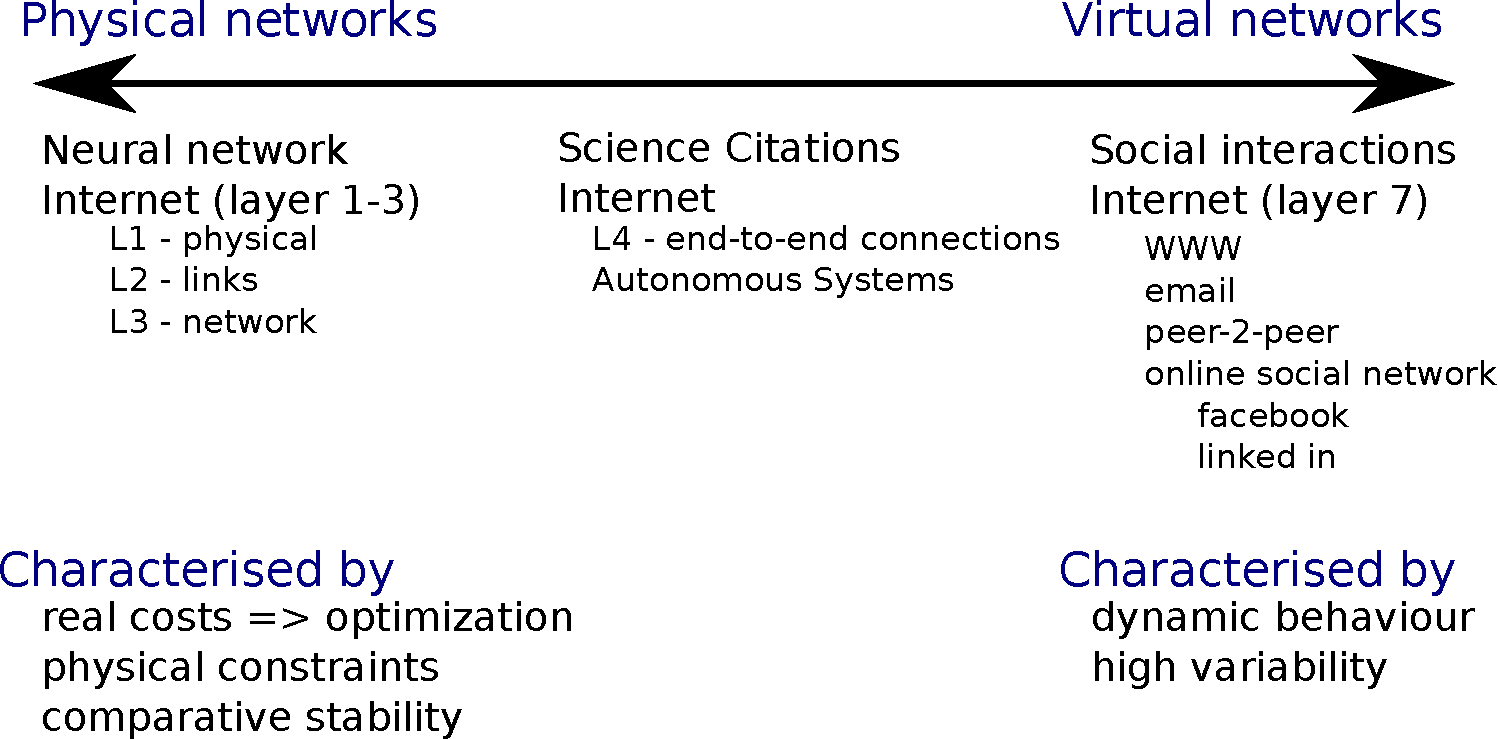
\includegraphics[width=1.1\figurewidth]{physical_vs_virtual.pdf}
    \caption{Physical vs virtual networks.\label{fig:phys_v_virt}}
  \end{center} 
\end{figure}


\item[Transport vs Information flows:] A more subtle differentiator
  is between what the network carries. Some networks physically
  transport some type of material (cars, water, ...) whereas the flows
  in other networks are (almost) pure information (the Internet,
  ...).  

  The importance of this distinction for networks may be less
  immediately obvious, but it certainly does have implications. When
  physical transport is involved in a network, the constraints on that
  network are likely to be even more stringent, and the ability to
  change the network even more limited. Costs for changing the road
  network, for instance, are usually higher than changing the
  equivalent proportion of a IP network.

\begin{figure}[htp]
  \begin{center}
     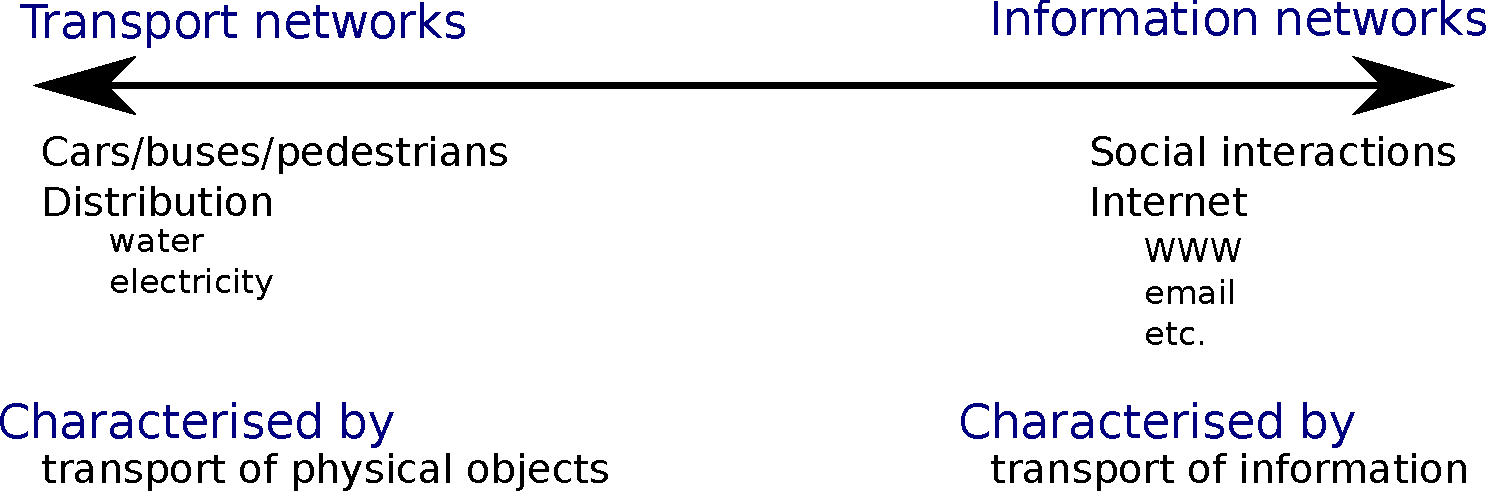
\includegraphics[width=1.1\figurewidth]{physical_vs_information.pdf}
 
    \caption{Transport vs information flows.\label{fig:trans_v_inf}}
  \end{center}
\end{figure}         

\end{description}
Within this chapter, we are primarily interested in the ``Internet'',
and that includes both physical (OSI layer 1-3) networks, and virtual
networks (MPLS, WWW, online social networks, etc.). However, all of
the networks considered here are information transportation networks.

There are other dimensions on which networks could be classified. For
instance, by the nature of the transport. Does it come in discrete
chunks (\eg cars, packets, or the post) or continuously (\eg water or
electricity)? Is the transport connection oriented (\eg the telephone
network) or packet oriented (\eg the Internet)?

And there are other general issues we need to deal with:
\begin{itemize}

  \item Physical networks are embedded in geography, but logical
    networks often aren't, and yet the same terminology is often
    applied to each.

  \item Connectivity often changes over time, with the time-scale
    varying depending on the type of network.

  \item The Internet is often said to be a ``network of networks''. It
    is often hard to consider one network in isolation, they have
    relationships, but the situations is even more complicated than
    often imagined.
    \begin{description}

    \item[peers] Networks may be connected to {\em peers}, \ie similar
      networks that may be competing or co-operating (or both in some
      cases), \eg two ISPs operating in the same region.

    \item[parents] Networks may have a parent-child relationship in
      the sense that one network controls the other, \eg the SS7
      network with respect to traditional telephone network.

    \item[layers] A single network may have multiple layers, each of
      which can be represented by a different graph, \eg the physical-
      vs the network-layers in the Internet.

    \item[external] There is substantial interaction between
      notionally separated networks, \eg the power grid and the
      Internet, both because the Internet uses electricity, but also
      because spikes in electricity demand could potentially be caused
      by network flash crowds (certainly TV programs have a very
      important impact on electricity usage).

    \end{description}
    
\end{itemize}

That brings us naturally to the particular object of discussion here
-- the Internet (and its topology).  The term ``Internet'' means
(many) different things to (many) different people.  Even within the
networking community, the term is often used ambiguously, leading to
misunderstandings and confusion and creating roadblocks for a
genuinely scientific treatment of an engineered system that has
revolutionized the way we live.

While mathematics in the form of graph theory has been equally
culpable in adopting the use of this vague nomenclature, the ``new
science of networks'' has popularized it to the point where phrases
like ``topology of the Internet'' or ``Internet graph'' have entered
the mainstream science literature, even though they are essentially
meaningless without precisely-stated definitions.  For one, ``Internet
topology'' could refer to the connectivity structures encountered in
any of layers in the protocol stack, or at various levels of
aggregation. Common examples are
\begin{enumerate}

\item {\bf Router-level (layer 3):} An often sought topology is the
  router level. Somewhat ambiguously, this may also be called the
  network level, or IP level, but ``network'' is a heavily overloaded
  term here, and the IP level can also be ambiguous. For instance, IP
  level could refer to the way IP addresses are connected, that is it
  could refer to the interfaces of one router as separate nodes
  \cite{broido01:_inter}, but that is rarely what is useful for
  network operations or research. We could also add at layer 3, in
  addition to {\em interface-level} topology described above, the {\em
    subnet-level} topology
  \cite{kardes12:_cheleb,gunes09:_resol_ip_inter,Tozal:2012:ENL:2342042.2342069,Tozal:tracenet:imc2010,broido01:_inter},
  describing the interconnectivity of logical subnets (often described
  by an IP-level prefix), but here we focus on the more commonly
  considered router level.

  The router-level graph shows a range of interesting implementation
  details of a network. This type of information is critical for
  network management applications, as much of Internet management
  rests at the IP layer, and it is of great importance for network
  adversaries. For instance, developing tools to measure network
  traffic requires an understanding of the router-layer topology, in
  order to match traffic to links. Similarly traffic engineering, and
  reliability analyses are carried out at this level. One complication
  of this layer is that we sometimes wish to obtain the topology
  extending out to end-hosts, which are not technically routers, but
  we shall include these in our definition of router-layer topology,
  unless otherwise specified.

\item {\bf Switch-level (layer 2):} A single IP layer logical link may
  hide several layer-2 devices (hubs and switches). The increasing
  prevalence of Ethernet, and the ability to provide redundancy at
  reasonable cost, has led to a proliferation of such devices, and
  most Local Area Networks (LANs) are based around such. Hence, very
  many networks which have trivial, or simple IP layer topologies have
  complex and interesting layer-2 topologies. Multi-Protocol Label
  Switching (MPLS) further complicates the situation by creating
  logical layer-2 networks without physical devices, often in the form
  of cliques. Measurements often see only one layer, creating
  misunderstandings of a network's true resilience and more general
  graph properties. For instance, layer-2 devices can connect large
  numbers of routers, making them appear to have higher degree at
  layer-3 \cite{Merindol:layer2:imc2010} (for more detailed discussion
  see \autoref{sec:mpls}).

\item {\bf Physical-level (layer 1):} Below the link layer (layer 2),
  lies the physical layer. Again, many physical devices may underly a
  single logical link. Discovery of this layer is of critical
  importance in network management tasks associated with
  reliability. In particular, the concept of Shared Risk Link Groups
  (SRLG) requires knowledge of which links are carried on which fibers
  (using Wavelength Division Multiplexing), in which conduits. If a
  backhoe digs up a single conduit, it will cause a bundle of fibers
  to fail, and so connections that are in the same SRLG will all fail
  simultaneously. Clearly redundant links need to be in different
  SRLG, and discovery of the physical topology is important to ensure
  that this is the case.

\item {\bf PoP-level:} A Point-of-Presence (PoP) is a loosely defined
  grouping of devices, often defined by a metropolitan area.  PoP
  level topologies are quite useful, essentially because these graphs
  describe the logical structure of the network as the designer
  intended, rather than its particular implementation in terms of
  individual routers. Such topologies are ideal for understanding
  tradeoffs between connectivity and redundancy, and also provide the
  most essential information to competitors or customers (about where
  a network is based, or who has the best access network in a
  region). Network maps are often drawn at this level because it is an
  easy level for humans to comprehend.

\item {\bf Application layer:} There has been significant interest in
  logical topologies of the application layer, \eg for the Web
  (using HTTP, and HTML), and the P2P applications. 
% We will not
%   consider such topologies in any detail here. Some approaches may be
%   similar, but by and large the approaches to determining these
%   topologies are very application dependent, \eg web crawlers for the
%   WWW.

\item {\bf AS-level:} AS topologies have generated much interest in
  the scientific literature~\cite{barabasi99,barabasi00,barabasi02},
  because they appear to show interesting properties (such as
  power-laws) in common with other un-engineered networks such as
  biological networks. Also, much data on AS topologies is publicly
  available. While of interest in the scientific literature, this
  data's use is confused by many myths and
  misunderstandings~\cite{roughan11}.  The data may provide mild
  competitive benefits, in allowing operators to determine who peers
  with who, but the measured data often comes without attributes that
  would make the data truly useful in this regard. Finally, it is hard
  to see how such data could be used in an attack, although much
  publicized reports such as \cite{barabasi02} suggest, incorrectly
  (see \cite{Li04}), that the observed structure of the AS graph may
  lead to an ``Achilles heel'' of the Internet.

  % \item {\bf Others:} There are other topologies that may be of
  % interest from time to time, for instance, that of a multicast
  % tree. 

\end{enumerate}
The number of possible topologies we might wish to discover highlights
the complexity of this problem, and why discovery is so valuable for
network management. In this chapter we will consider the router-level
topology in detail, and then discuss some of the similarities and
differences with respect to AS- and PoP-level topologies.

In addition to understanding the Internet network as a simple graph,
there are many other features of the graph that one would also wish to
know, for instance, its routing, link capacities, and geographic
locations. We describe such qualities as graph attributes, and find
that most can either be attributed to edges of the graph, for instance
\begin{sitemize} 

  \item link capacities,

  \item link length,
 
  \item routing weights (\eg for shortest-path routing),

  \item link utilizations,

  \item link performance (for example, bit-error-rate, delay, loss,
  jitter, reordering, buffer utilization), 

  \item link status (up/down), and 

  \item a link's lower layer properties (\eg number of physical hops),

\end{sitemize}
or to the nodes of the graph
\begin{sitemize}

  \item geographic location,

  \item type of node, \eg brand of router, or version of software,

  \item performance measures (\eg CPU utilization), and 

  \item node status (up/down).

\end{sitemize}
We could further divide this list into \define{intrinsic} network
properties, such as node location, or link capacity (things that
cannot change easily), and \define{extrinsic} properties, such as
performance, or traffic related properties, which can change
dramatically despite there being no change in the underlying network.

% In a few cases, it is hard to attribute a quality to an individual
% component of the network. For instance, routing in a network is often
% of interest. In the case of shortest path routing, this can be
% completely characterized by simple link weight attributes for each
% link, but many networks use routing protocols to create more complex
% routings. This type of complexity can sometimes be simply described by
% simple attributes, but may in other cases may be rather more
% difficult. For example OSPF with areas is often used to create a type
% of hierarchy within an AS --- in this example we can still use link
% attributes because we can assign an OSPF area to each link, but the
% attributes may be more difficult to measure. In other cases, for
% example if BGP was used as an IGP to create policy based routing
% internally in a network, we cannot describe the routing with simple
% attributes (to some extent the routing could still be captured by the
% forwarding table, which is an extreme example of a router attribute,
% but we shall exclude such extreme cases of attributes for the
% moment.). In these cases, the attributes really belong to end-to-end
% paths through the network, keyed on IP addresses (source and
% destination). We shall not consider such attributes in this report,
% though they may be of interest.

%% As an example of how one might use attributes: given node locations, it
%% is trivial to build a PoP level topology from a router-level topology.


%\clearpage
\section{Router-level topology}
\label{sec:router}

\subsection{A look back}
\label{sec:router_hist}

Since the early days of the ARPANET, networking researchers have been
interested in drawing the type of networks they
designed~\cite{heart78:_arpanet}.  An early map of the ARPANET is
reproduced in \autoref{fig:arpa_1971} and shows the network's logical
connectivity structures in April 1971, when the network as a whole
consisted of some 15 nodes and a node was little more than one or two
state-of-the-art computers connected via an Interface Message
Processor or IMP (the modern equivalent would be a router).  In this
context, logical structure refers to a detailed drawing of the
connectivity among those nodes and of node-specific details (\eg type
of machine), by and large ignoring geography.  In contrast, geographic
structure refers to a map of the US that includes the actual locations
of the network's physical nodes and shows the physical connectivity
among those nodes. Such accurate maps could be drawn because at that
time, each piece of equipment was expensive and needed to be accounted
for, only a few groups with a small number of researchers were
involved in the design and installation of the network, and the
network changed relatively slowly.

\begin{figure}[thbp]
  \begin{center}
    \begin{subfigure}[b]{0.75\textwidth} \centering
      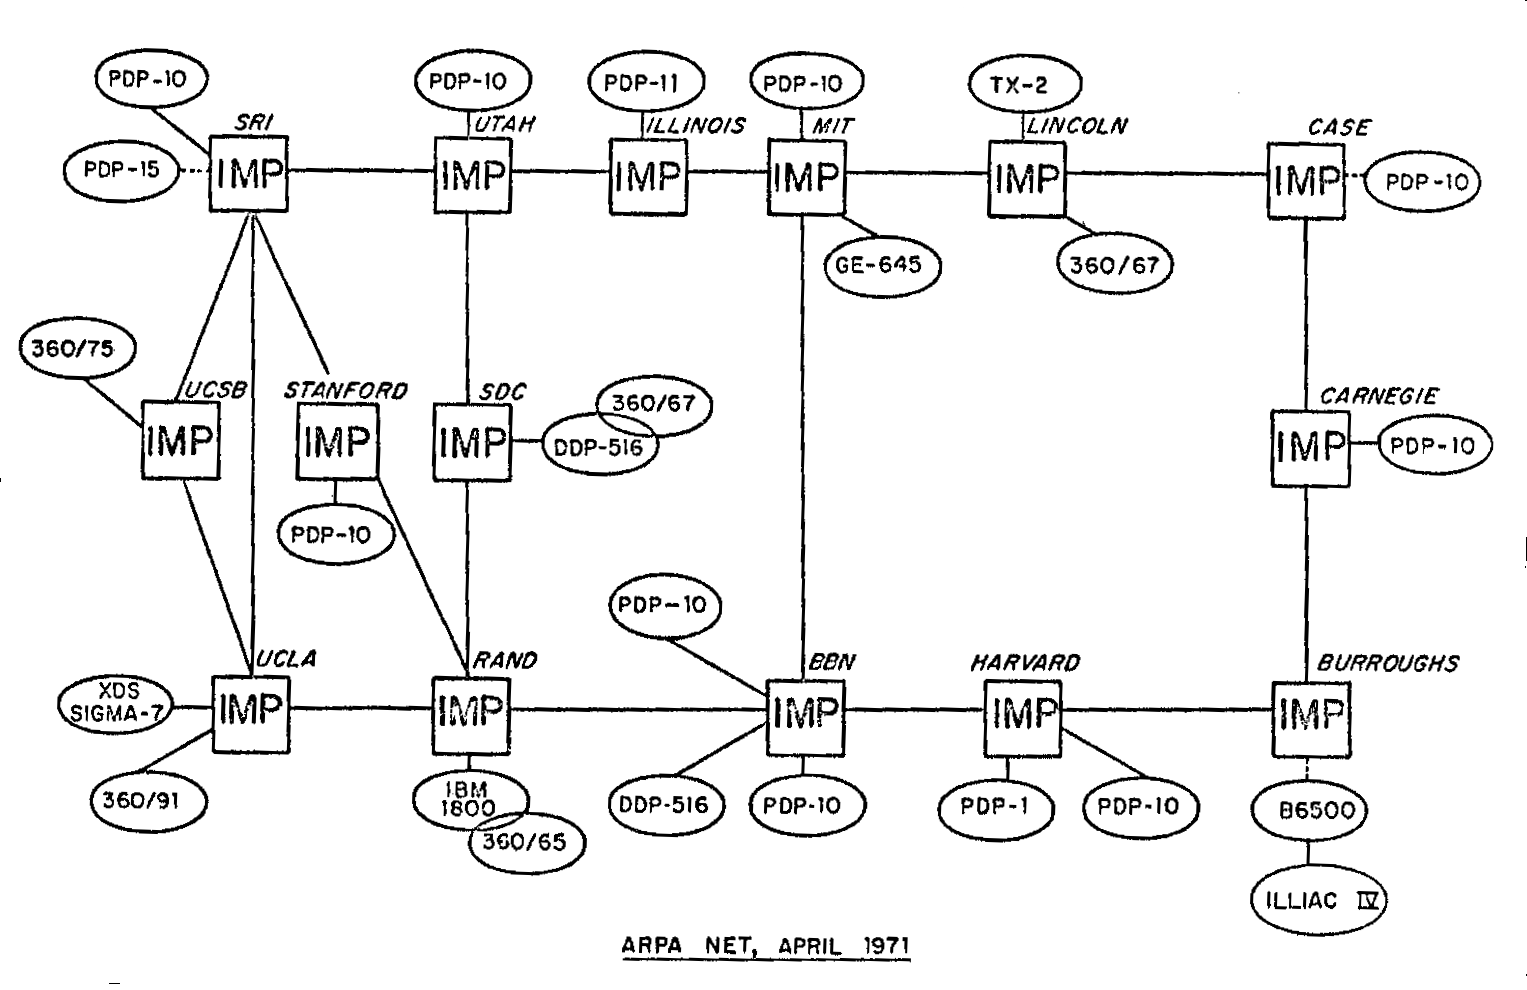
\includegraphics[width=1\textwidth]{cerf_arpanet_1971_april.png}
    \end{subfigure}
    \caption{The ARPANET in 1971 (reprinted from
      \cite{cerf90:_selected_maps}; \copyright 1990 ACM, Inc. Included here by permission.)
      \label{fig:arpa_1971}}
% \url{http://www.cs.utexas.edu/users/chris/DIGITAL_ARCHIVE/ARPANET/DARPA4799.pdf}
% (page III-144, page III-81)
  \end{center}
\end{figure}


\begin{figure}[thbp]
  \begin{center}
    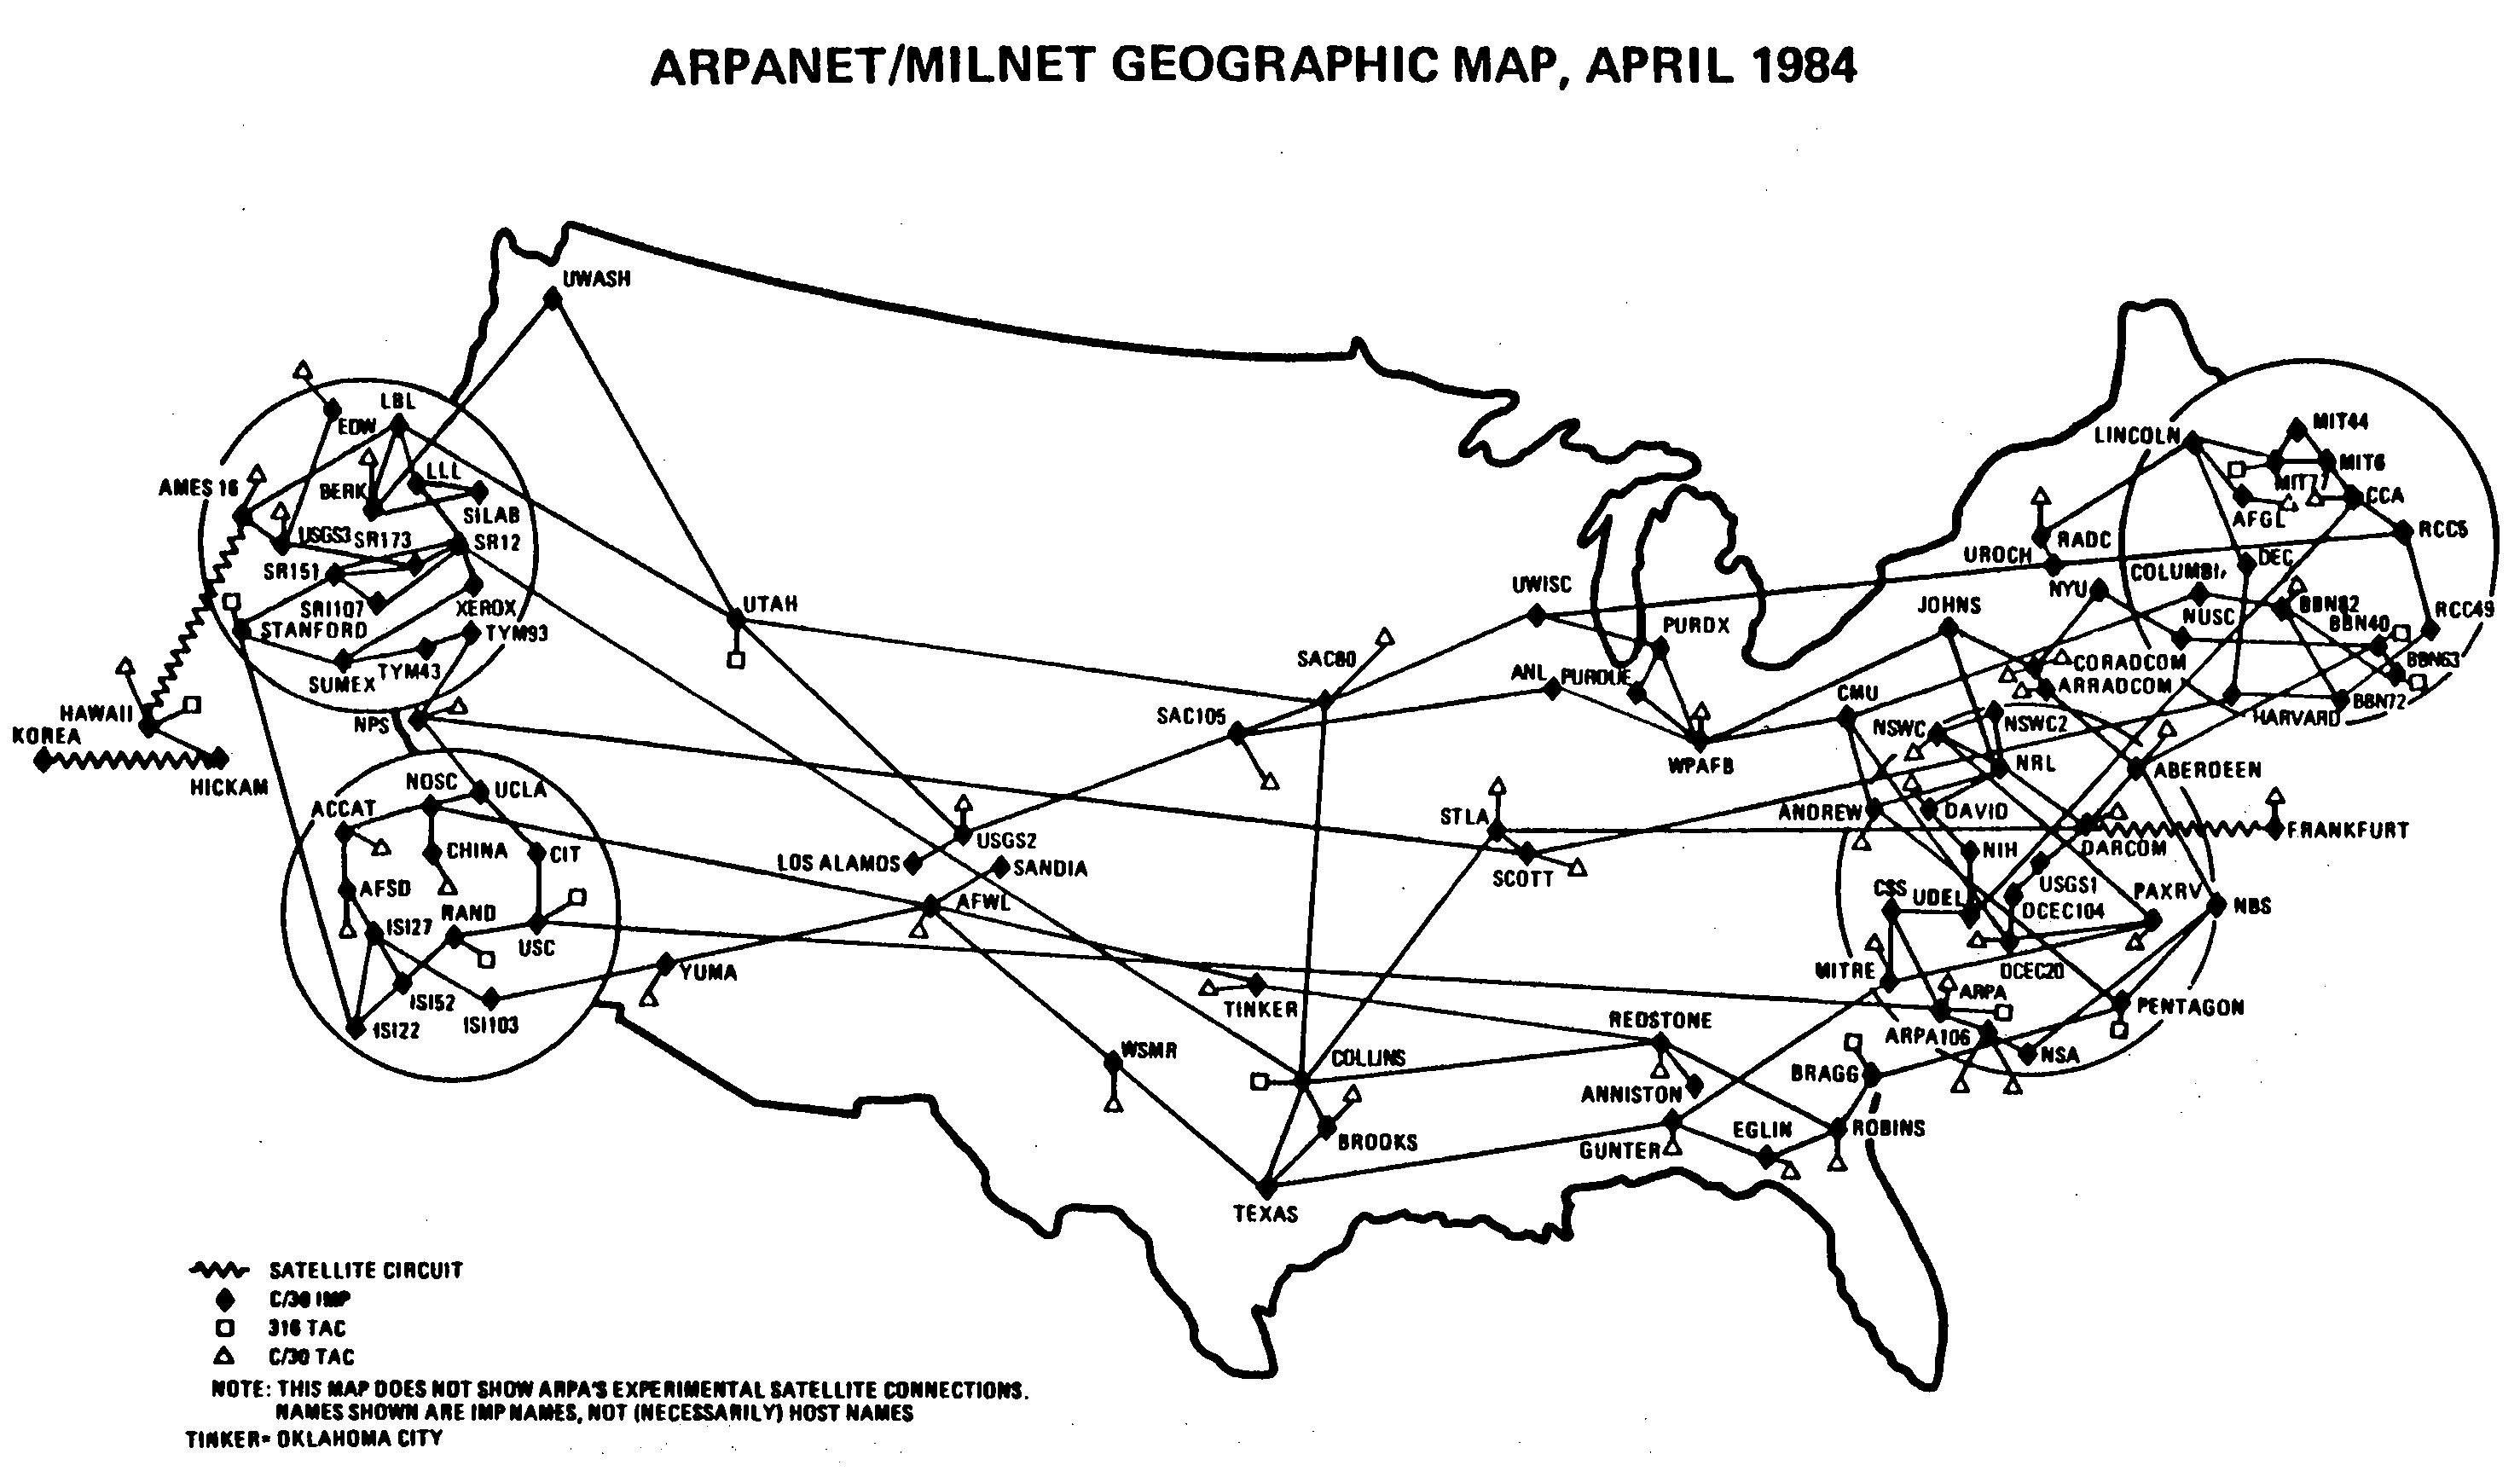
\includegraphics[width=0.9\textwidth]{cerf_arpanet_1984.png}
    \caption{The early ARPANET  (reprinted from
      \cite{cerf90:_selected_maps}; \copyright 1990 ACM, Inc. Included here by permission.)
      \label{fig:arpa_1984}}
  \end{center}
\end{figure}

The network quickly grew in size and complexity. For instance,
\autoref{fig:arpa_1984} shows the geographic counterpart from 1984 of
the ARPANET map depicted in \autoref{fig:arpa_1971}.  Manually
accounting for the increasing number of components quickly became
prohibitive and motivated the adoption of automatic strategies for
obtaining some of the available connectivity as well as traffic
information.  A prime example for effectively visualizing this
collected information is reproduced from
\cite{frazer:_merit_histor_nsfnet_backb_projec} and shown in
\autoref{fig:nsfnet}, which depicts a 3D rendering of the (US portion
of the) NSFNET around 1991, annotated with traffic-related
information. At that time, the NSFNET backbone consisted of some 14
nodes that were interconnected with T1 links as shown and, in turn,
connected to a number of different campus networks (\eg collections of
interconnected LANs). However, even though the internal structure of
the backbone nodes was well-known (\ie each node was composed of nine
IBM RTs linked by two token rings with an Ethernet interface to
attached networks), nobody had any longer access to the internals of
all the different campus networks and as a result, drawing the 1991
NSFNET equivalent of the ARPANET's logical connectivity structure
(\autoref{fig:arpa_1971}) was no longer possible.
 
\begin{figure}[thbp]
  \begin{center}
    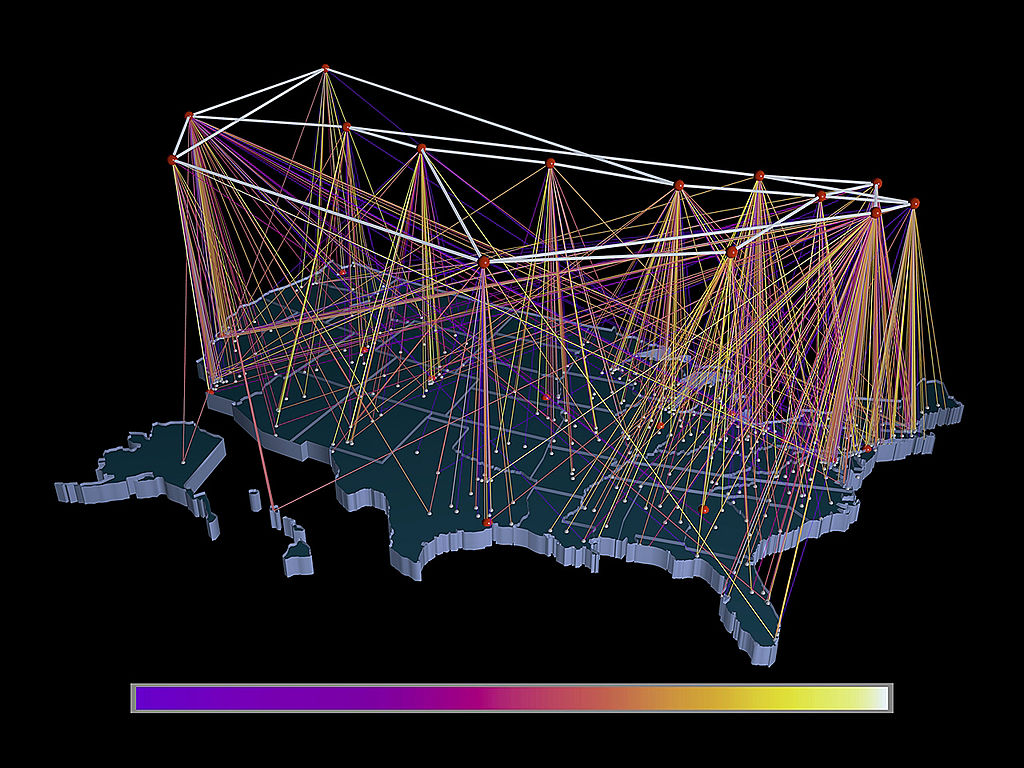
\includegraphics[width=0.7\textwidth]{1024px-NSFNET-traffic-visualization-1991.jpg}
    \caption{A visualization of the NSFNET circa 1991 (by Donna Cox
and Robert Patterson,
\href{http://avl.ncsa.illinois.edu/project-archive/visualizing-the-early-internet}{National
Center for Supercomputing Applications, University of Illinois at
Urbana-Champaign}. See also
\url{http://en.wikipedia.org/wiki/File:NSFNET-traffic-visualization-1991.jpg}).
      \label{fig:nsfnet}}
  \end{center}
\end{figure}

With the decommissioning of the NSFNET in 1995 and the rise of the
"public Internet", the researchers' ability to obtain detailed
connectivity and component information about the internals of the
different networks that formed the emerging "network of networks"
further diminished and generated renewed interest in the development of
abstract, yet informed, models for router-topology evaluation and
generation. For example, the Waxman model \cite{Waxman88}, a variation
of the classical Erd\"{o}s-R\'{e}nyi random graph model \cite{erdos60}
was the first popular topology generator commonly-used for network
simulation studies at the router level. However, it was largely
abandoned in the late 1990s in favor of models that attempted to
explicitly account for non-random structure as part of the network
design. The arguments that favored structure over randomness were
largely empirical in nature and reflected the fact that the inspection
of real-world router-level ISP networks showed clear signs of
non-random structures in the form of the presence of backbones, the
appearance of hierarchical designs, and the importance of locality.
These arguments also favored the notion that a topology generator
should reflect the design principles in common use; \eg to achieve
some desired performance objectives, the physical networks must
satisfy certain connectivity and redundancy requirements, properties
which are generally not guaranteed in random network topologies.
These principles were, for example, advanced in
\cite{Zegura96,Calvert97,Zegura97} and were ultimately integrated into
the popular Georgia Tech Internetwork Topology Models (GT-ITM)
\cite{gt_itm}.
 
These more structure-oriented router topology generators were viewed
as the state-of-the-art until around 2000 when, in turn, they were
largely abandoned in favor of a new class of random graph models whose
trademark was the ability to reproduce the newly discovered power-law
relationship in the observed connectivity (\ie node degree) of
router-level graphs of the Internet. This discovery was originally
reported in the seminal paper by
Faloutsos~\etal~\cite{faloutsos99:_power_law_relat_of_inter_topol},
who used a router-level graph constructed from data that was collected
a few years earlier by Pansiot and Grad~\cite{pansiot98:_inter} for
the purpose of obtaining some experimental data on the actual shape of
multicast trees in the Internet. The Boston university Representative
Internet Topology gEnerator (BRITE) \cite{Medina01} became a popular
representative of this new class of models, in part also because it
combined the more structure-oriented perspective of the GT-ITM
generator with the new focus that emphasized the ability to reproduce
certain metrics or statistics of measured router topologies (\eg node
degree distribution).

One of the hallmarks of networks that have power-law degree
distributions and that are generated according to any of a number of
different probabilistic mechanisms (\eg preferential attachment
\cite{barabasi99}, random graphs with a given expected degree sequence
\cite{Chung04}, power-law random graphs 
\cite{Aiello00}) is that they can be shown to have
a few centrally located and highly connected {\em hubs} through which
essentially most traffic must flow.  When using these models to
represent the router-level topology of the Internet, the presence of
these highly connected central nodes has been touted the Internet's
``Achilles-heel'' because network connectivity is highly vulnerable to
attacks that target the high-degree hub nodes \cite{barabasi00}. It has been
similarly argued that these high-degree hubs are a primary reason for
the epidemic spread of computer worms and viruses \cite{berger05:_spread_of_viruses,pastor-satorras01:_epidem}.
Importantly, the presence of highly connected central nodes in a
network having a power-law degree distribution is the essence of the
so-called scale-free network models. They have been a highly popular
theme in the study of complex networks, particularly among researchers
inspired by statistical physics \cite{albert_barabasi02}, and have fuelled the rise of
a new scientific discipline that has become known as ``Network
Science" \cite{barabasi12}.  In the process, they have also seen wide-spread
use among Internet topology researchers.

However, as the general fascination with and popularity of network
science in general and scale free network modeling in particular grew,
so did the arguments that were voiced by Internet researchers
and questioned the appropriateness and relevance of the scale-free
modeling approach for studying highly-engineered systems such as the
Internet's router topology. In fact, at around 2010, when the number
of publications in the area of network science reached a new height,
the number of papers that were published in the networking research
literature and applied scale-free network models to describe or study
router-level topologies of the Internet was close to zero.  This begs
the question ``What happened?'', and the answer provided in the next
section is really a classic lesson in how errors of various forms
occur and can add up to produce results and claims that create
excitement among non-networking researchers, but quickly collapse when
scrutinized with real data or examined by domain experts.



\subsection{Know your measurements}
\label{sec:router_measurements}

Between 1990 and 2000, Internet topology research underwent a drastic change from being
a data-starved discipline to becoming a prime example of a largely measurement-driven research 
activity.  As described earlier, even though the development of abstract, yet informed,
models for network topology evaluation and generation has always been a give and take between
theoreticians and empiricists, for router topology modeling, the essential role that
measurements have started to play came into full focus in a sequence of three seminal papers that
appeared between 1998-2000. 

\subsubsection{Three seminal papers on router topology modeling}
\label{sec:router_seminal}

The key papers that turned router topology modeling into a full-fledged measurement-driven
research activity cover the whole spectrum of modeling activities, from
measurement experiments to model construction and validation to graph-theoretical network
analysis, and are listed below: 

\begin{itemize}
\item[(i)] ``On routes and multicast trees in the Internet'' by
  J.-J. Pansiot and D. Grad (1998) \cite{pansiot98:_inter} described
  the original measurement experiment that was performed in mid-1995
  and produced data on actual routes taken by packets in the
  Internet. This data was subsequently used to construct a router
  graph of the Internet.

\item[(ii)] ``On power-law relationships of the Internet topology'' by
  M. Faloutsos~\etal~(1999)
  \cite{faloutsos99:_power_law_relat_of_inter_topol} reported (among
  other observations) on the observed power-law relationship in the
  connectivity of the router-level topology of the Internet measured
  by Pansiot and Grad~\cite{pansiot98:_inter}.

\item[(iii)] ``Error and attack tolerance of complex networks'' by
  R. Albert~\etal~(2000) \cite{barabasi00} proposed a scale-free
  network model to describe the router topology of the Internet and
  argued for its validity on the basis of the latest findings by
  Faloutsos~\etal~\cite{faloutsos99:_power_law_relat_of_inter_topol}.
  It touted the new model's exemplary predictive power by reporting on
  the discovery of a fundamental weakness of the Internet (a property
  that was became known as the Internet's "Achilles' heel") that went
  apparently unnoticed by the engineers and researchers who have
  designed, deployed, and studied this large-scale, critical
  infrastructure, but followed directly from the newly proposed
  scale-free modeling approach.
\end{itemize}

\begin{figure}[!htp] 
  \begin{center}
    \includegraphics*[width=0.8\columnwidth,viewport=0mm 52mm 260mm 160mm]{ams-figs-final.pdf}
    \caption{A toy example of a scale-free network of the preferential
      attachment type (b) generated to match a power-law type node
      degree distribution (a).  (First published in Notices of the
      American Mathematical Society, Volume 56, No.3 (May 2009):
      586-599 \cite{willinger09:_mathem_and_inter}. Included here by
      permission.)
      \label{fig:hot_1}}
    % \url{http://www.ams.org/notices/200905/rtx090500586p.pdf}  (figure 1)
  \end{center}
\end{figure}         


At first glance, the combination of these three papers appears to show
network modeling at its best -- firmly based on experimental data,
following modeling practices steeped in tradition, and discovering
surprisingly and previously unknown properties of the modeled network.
An example of a toy network resulting from taking the findings from
these seminal papers at face value is shown in \autoref{fig:hot_1}.
However, one of the beauties of studying man-made systems such as the
Internet is that -- because of their highly-engineered architectures,
a thorough understanding of its component technologies, and the
availability of extensive (but not necessarily very accurate)
measurement capabilities -- they provide a unique setting in which
most claims about their properties, structure, and functionality can
be unambiguously resolved, though perhaps not without substantial
efforts. In the remainder of this section, we will illustrate how in
the context of the Internet's router topology, applying readily
available domain knowledge in the form of original design principles,
existing technological constraints, and available measurement
methodologies reveals a drastically different picture from that
painted in these three seminal papers. In fact, we will expose the
specious nature of scale-free network models that may appeal to more
mathematically inclined researchers because of their simplicity or
generality, but besides having no bearing on the Internet's router
topology are also resulting in wrong claims about the Internet as a
whole.


\subsubsection{A first sanity check: Using publicly available information}



A first indication of apparent inconsistencies between the proposed
scale-free models for the Internet's router topology and the actual
Internet comes from the inspection of the router topologies of actual
networks that make the details of their network internals publicly
available. For example, networks such as Internet2~\cite{internet2} or
G\'{E}ANT~\cite{geant} show no evidence that there exist any centrally
located and highly connected ``hubs'' through which essentially most
traffic must flow.  Instead, what they typically show is the presence
of a more or less pronounced ``backbone'' network that is fed by
tree-like access networks, with additional connections at various
places to provide a degree of redundancy and robustness to components
failures\footnote{This is not a universal phenomena. For instance
  \cite{Zoo} notes that some networks do exhibit hub-like structure, but
  it is the lack of universality that is important here, as exhibited
  by these and other counter examples.}.

This design pattern is fully consistent with even just a cursory
reading of the most recent product catalogs or white papers published
by the main router vendors
\cite{cisco13:_build_cost_effec_scalab_core,cisco13:_converged,juniper13:_evolv_backb_networ_using_mpls_super}.
For one, the most expensive and fastest or highest-capacity pieces of
equipment are explicitly marketed as backbone routers. Moreover, due
to inherent technological limitations in how many packets or bytes a
router can handle in a given time interval, even the latest models of
backbone routers can support only a small number of very
high-bandwidth connections, typically to connect to other backbone
routers. At the same time, a wide range of cheaper, slower or
lower-capacity products are offered by the different router vendors
and are targeted primarily at to support network access.  On the
access side, a typical router will have many lower-bandwidth
connections for the purpose of aggregating customer traffic from the
network's edge and subsequently forwarding that traffic towards the
backbone. In short, even the latest models advertised by today's
router vendors are limited by existing technologies, and even for the
top-of-the-line backbone routers, it is technologically infeasible to
have hundreds or thousands of high-bandwidth connections. At the same
time, while technically feasible, deploying some of the most expensive
equipment and configuring it to support hundreds or thousands of
low-bandwidth connections would be considered an overall bad
engineering decision (\eg excessively costly, highly inefficient, and
causing serious bottlenecks in the network).
 
However, the root cause for these outward signs of a clear mismatch
between the modeled and actual
router topology of the Internet goes deeper and lies in the original design philosophy of the
Internet.  As detailed in \cite{clarke95:_design}, while the top level goal for the original DARPA Internet architecture was {\it ``to develop an effective technique for multiplexed utilization
of existing interconnected networks"}, the requirement that {\it ``Internet communication must
continue despite loss of networks or gateways"} topped the list of second level goals. To survive
in the face of components failing off, the architecture was to mask completely any transient 
failure, and to achieve this goal, state information which describes an existing connection must
be protected. To this end, the architecture adopted the ``fate-sharing" model that gathers this 
state information at the endpoints of connections, at the entities that are utilizing the 
service of the network. Under this model, it is acceptable to lose the state information 
associated with an entity if, at the same time, the entity itself is lost; that is, there 
exists no longer any physical path over which any sort of communication with that entity can
be achieved (\ie total partition). Ironically, these original design principles
outlined in \cite{clarke95:_design} favor precisely the opposite of what the scale-free modeling approach
yields -- no centrally located and highly connected ``hubs'' because their removal makes
partitioning the network easy.


\subsubsection{An in-depth look at traceroute: \\ Examining a popular measurement technique}
\label{sec:mpls}

While the above-mentioned empirical, technological, and architectural
arguments cast some serious doubts on the scale-free network modeling
approach for the router topology of the Internet, they say nothing
about the measurements that form the basis of this approach and has
given it a sense of legitimacy among scientists in general and
networking researchers in particular.  To appreciate the full role
that measurements play in this discussion, it is informative to
revisit the original paper by Pansiot and Grad~\cite{pansiot98:_inter}
that describes the measurement experiment, discusses the measurement
technique used, and provides a detailed account of the quality of the
data that form the basis of the scale-free approach towards modeling
the Internet's router topology.

In essence, \cite{pansiot98:_inter} describes the first (at that time)
large-scale traceroute campaign performed for the main purpose of
constructing a router graph of the Internet from actual Internet
routes. Although traceroute-based, the authors of
\cite{pansiot98:_inter} quickly point out that their purpose of using
the traceroute tool (\ie obtaining actual Internet routes to
construct a router graph) differed from what V. Jacobson
\cite{jacobson89:_tracer} had in mind when he originally designed the
tool (\ie tracing a route from a source to a destination for
diagnostic purposes).  As a result, a number of serious issues arise
that highlight why using the traceroute technique for the purpose of
constructing a router graph is little more than an "engineering hack"
and can certainly not be called a well-understood "measurement
methodology."

{\bf IP alias resolution problem:} One serious problem
explained in detail in \cite{pansiot98:_inter} with using traceroute-based data for
constructing router graphs is that the traceroute tool only returns
the IP addresses of the interface cards of the routers that the probe
packets encountered on their route from the source to their
destination.  However, most routers have many interface cards, and
despite many years of research efforts that have produced a series of
increasingly sophisticated heuristics \cite{bender08:_fixin_allys,gunes09:_resol_ip_inter,sherry10:_resol_ip_alias_presp_times}, the networking
community still lacks rigorous and accurate methods for resolving the
IP alias resolution problem; that is, determining whether two
different interface IP addresses belong to or can be mapped to the
same router. While the essence of this problem is illustrated in
\autoref{fig:hot_2}, the impact it can have when trying to map a
router topology of an actual network is shown in \autoref{fig:hot_3}.


\begin{figure}[!htp] 
  \begin{center}
% pdfimages gets actual 'images' (bitmaps) out of the PDF, but not plots
% pdfjam ams-figs-final.pdf '5' --outfile ams-figs-p5.pdf
%     extracts a particular page so I can use it here
    \includegraphics*[width=0.6\columnwidth,viewport=10mm 110mm 200mm 200mm]{ams-figs-p2.pdf}
%                                                    xleft ybottom xright ytop
%                                                 a4 = 0 0 210 297
    \caption{The IP alias resolution problem. Paraphrasing Fig. 4 of \cite{rocketfuel_1}, 
	 traceroute does not list routers (boxes) along paths but IP addresses of 
	 input interfaces (circles), and alias resolution refers to the correct 
	 mapping of interfaces to routers to reveal the actual topology. In the case
	 where interfaces 1 and 2 are aliases, (b) depicts the actual topology while 
	 (a) yields an ``inflated'' topology with more routers and links.
	 (First published in Notices of the American Mathematical Society, Volume 56, 
	 No.3 (May 2009): 586-599 \cite{willinger09:_mathem_and_inter}. Included here by permission.)
      % \cite[Figure~2]{willinger09:_mathem_and_inter}.
      \label{fig:hot_2}}
    % \url{http://www.ams.org/notices/200905/rtx090500586p.pdf}  (figure 2)
  \end{center}
\end{figure}         

\begin{figure}[thbp] 
  \begin{center}
% pdfimages gets actual 'images' (bitmaps) out of the PDF, but not plots
% pdfjam ams-figs-final.pdf '5' --outfile ams-figs-p5.pdf
%     extracts a particular page so I can use it here
    \includegraphics*[width=1\columnwidth,viewport=0mm 70mm 210mm 240mm]{ams-figs-p3.pdf}
%                                                    xleft ybottom xright ytop
%                                                 a4 = 0 0 210 297
    \caption{The IP alias resolution problem in practice. Shown is a comparison 
	 between the Abilene/Internet2 topology inferred by Rocketfuel (left) and the 
	 actual topology (top right). Rectangles represent routers with interior ovals 
	 denoting interfaces. The histograms of the corresponding node degrees are 
	 shown in the bottom right plot. 
	 (Reprinted from \cite{sherwood08:_discar}; \copyright 2008
         ACM. Inc. Included here by permission.)
         \label{fig:hot_3}}
    % \url{http://www.ams.org/notices/200905/rtx090500586p.pdf}  (figure 3)
  \end{center}
\end{figure}         

\clearpage
{\bf Lesson 1:} {\em Due to the absence of accurate and rigorous methods for solving the IP alias
resolution problem, the actual values of the connectivity of each router (\ie node degrees)
inferred from traceroute measurements cannot be taken at face
value.}

{\bf Opaque Layer-2 clouds:} Another serious issue with
using generic traceroute-based measurements for construction router
graphs is also discussed at length in \cite{pansiot98:_inter} and
illustrated in \autoref{fig:hot_4}.  Being strictly limited to IP or
layer-3, the problem with traceroute is that it is incapable of
tracing through opaque layer-2 clouds that feature circuit
technologies such as Asynchronous Transfer Mode (ATM) or Multiprotocol
Label Switching (MPLS). These technologies have the explicit and
intended purpose of hiding the network's physical infrastructure from
IP, so from the perspective of traceroute, a network that runs these
technologies will appear to provide direct connectivity between
routers that are separated by local, regional, national, or even
global physical network infrastructures. An example of using
traceroute to map a network that uses MPLS is depicted in
\autoref{fig:hot_4} and shows an essentially completely connected
graph at Layer 3 with multiple high-degree nodes, even though the
physical router topology is very sparse. Similarly, if traceroute
encounters an ATM cloud, it falsely ``discovers'' a high-degree node
that is really a logical entity -- often an entire network potentially
spanning many hosts or great distances -- rather than a physical node
of the Internet's router-level
topology. Donnet~\etal~\cite{benoit12:_reveal_mpls} found that at
least 30\% of the paths they tested traversed an MPLS tunnel.

Recent extensions of the ICMP protocol, using traceroute to trace
through opaque MPLS clouds have become technically
feasible~\cite{rfc4950}, but operators often configure their routers to
hide the MPLS tunnels by turning off this option
\cite{sommers11:_preval_charac_mpls_deploy_open_inter}. Even then it
may be possible to detect the MPLS tunnels
\cite{benoit12:_reveal_mpls}, but the inference techniques are not a
guarantee, and are quite particular to MPLS, which is not the only
technique for creating tunnels, so there may still be some opaque
networks to deal with.  More to the point, even where such inferences
are possible, most data sets do not contain this type of analysis, and
most subsequent analyses of the data have ignored the issue.


\begin{figure}[thbp] 
  \begin{center}
% pdfimages gets actual 'images' (bitmaps) out of the PDF, but not plots
% pdfjam ams-figs-final.pdf '5' --outfile ams-figs-p5.pdf
%     extracts a particular page so I can use it here
    \includegraphics*[width=1\columnwidth,viewport=17mm 70mm 193mm 240mm]{ams-figs-p4.pdf}
%                                                    xleft ybottom xright ytop
%                                                 a4 = 0 0 210 297
    \caption{How traceroute detects fictitious high-degree nodes in
      the network core. (a) The actual connectivity of an opaque
      layer-2 cloud, i.e., a router-level network running a technology
      such as ATM or MPLS (left) and the connectivity inferred by
      traceroute probes entering the network at the marked router
      (right).  (b) The Rocketfuel-inferred backbone topology of
      AS3356 (Level3), a Tier-1 Internet service provider and leader
      in the deployment of MPLS.  (Figure (b) reprinted from \cite{rocketfuel_1};
      \copyright 2002 ACM, Inc. Included here by permission.)
       % \cite[Figure 4]{willinger09:_mathem_and_inter}.
      \label{fig:hot_4}}
    % \url{http://www.ams.org/notices/200905/rtx090500586p.pdf}  (figure 4)
  \end{center}
\end{figure}         

{\bf Lesson 2:} {\em Due to an inability of the generic traceroute
technique to trace through opaque Layer-2 clouds, or understand the
connectivity created by Layer-2
devices~\cite{Merindol:layer2:imc2010}, the inferred high-degree nodes
(\ie routers with a large number of connections) are typically
fictitious, an artifact of an imperfect measurement tool.}

{\bf Limited vantage points:} We have commented earlier
that since a router is fundamentally limited in terms of the number of
packets it can process in any time interval, there is an inherent
tradeoff in router configuration: it can support either a few
high-throughput connections or many low-throughput connections. Thus,
for any given router technology, a high-connectivity router in the
core reflects a poor design decision -- it will either have poor
performance due to its slow connections or be prohibitively expensive
relative to other options. Conversely, a good design choice is to
deploy cheap high-degree router near the edge of the network and rely
on the very technology that supports easy multiplexing of a large
number of relatively low-bandwidth links. Unfortunately, neither the
original traceroute-based study of Pansiot and
Grad~\cite{pansiot98:_inter} nor any of the larger-scale campaigns
that were subsequently performed by various network research groups
have the ability to detect those actual high-degree nodes. The simple
reason is that these campaigns lack access to a sufficient number of
vantage points (\ie sources for launching traceroute probes and
targets) in any local end-system to reveal these actual high
connectivity patterns at the network's edge.

{\bf Lesson 3:} {\em If there were high-degree nodes in the network,
existing router technology relegates them to the edge of the network
where no generic traceroute-based measurement campaigns is able to
detect them because of a lack of vantage points nearby.}

There are other issues with large-scale traceroute campaigns that
impact the quality of the resulting measurements and have received
some attention in the literature.  For example, the use of traceroute
has been shown to make experimental data susceptible to a type of
measurement bias in which some nodes of the network are oversampled,
while others are undersampled. However, while this feature has
received considerable attention
\cite{LakhinaByersCrovellaXie03,achlioptas05:_bias_of_tracer_sampl},
in the presence of systematic errors due to an inability to perform
accurate IP alias resolution or trace through opaque Layer-2 clouds,
this work is largely of theoretical interest and of little practical
relevance for modeling the Internet's router topology.



% \noindent {\bf Efficiency:} reducing the number of packets --


% "Efficient IP-level Network Topology Capture" [Paper]
% Bourgeau Thomas (UPMC Sorbonne Universities)
% Timur Friedman (UPMC Sorbonne Universities)
% PAM 2013


\subsubsection{Just the facts: power-law scaling and router-level topologies}

When applying lessons 1-3 to the main findings reported in the seminal
papers discussed in \autoref{sec:router_seminal} we are faced with the
following facts:
\begin{description}
\item[{\bf Fact 1:}] A very typical but largely ignored fact about Internet-related 
measurements in general and traceroute measurements in particular is that what we can 
measure in an Internet-like environment is generally not the same as what we really 
want to measure (or what we think we actually measure). This is mainly because as a 
decentralized and distributed system, the Internet lacks a central authority and does 
not support third-party measurements.

\item[{\bf Fact 2:}] A particularly ironic fact about traceroute is that the high-degree nodes 
it detects in the network core are necessarily fictitious and represent entire opaque 
layer-2 clouds, and if there are actual high-degree nodes in the network, existing technology
relegates them to the edge of the network where no generic traceroute-based measurement
experiment will ever detect them.

\item[{\bf Fact 3:}] In particular, due to the inherent inability of traceroute to (i) reveal 
unambiguously the actual connectivity (\ie node degree) of any router, and (ii) correctly 
identify even the mere absence or presence of high-degree nodes (let alone their actual values),
statistical statements such as those made in \cite{faloutsos99:_power_law_relat_of_inter_topol} claiming that the Internet's router 
connectivity is well described by  a power-law distribution (or, for that case, any other type of distribution) cannot be justified with any reasonable degree of statistical confidence.

\item[{\bf Fact 4:}] Since historical traceroute-based measurements cannot be taken at 
face value when (mis)using them for inferring router topologies and the inference results 
obtained from such data cannot be trusted, the claims that have been made about the 
(router-level) Internet in \cite{barabasi00} are without substance and collapse under careful scrutiny.
\end{description}
 
In short, after almost 15 years of examining the idiosyncrasies of the traceroute tool,
there exists overwhelming evidence that the sort of generic and raw traceroute measurements
that have been used to date to infer the Internet's router topology are seriously flawed to 
the point of being essentially of no use for performing scientifically sound inferences. 
Yet, the myth that started with 
\cite{faloutsos99:_power_law_relat_of_inter_topol}; \ie the router topology of the Internet exhibits 
power-law degree distributions persists and continues to be especially popular with researchers 
that typically work in the field of network science and show in general little interest in 
domain-specific "details" such as traceroute's idiosyncrasies.

At the same time, it is worthwhile pointing out that most of the
above-mentioned flaws and shortcomings of traceroute-based
measurements are neither new nor controversial with networking
researchers.  In fact, when discussing the use of the traceroute tool
as part of their original measurement experiment, the authors of  \cite{pansiot98:_inter} described many of the issues
discussed in this section in great detail and commented on the
possible implications that these inherently traceroute-related issues 
can have for constructing router graphs of the Internet. In this
sense, \cite{pansiot98:_inter} is an early example of an exemplary measurement paper,
but unfortunately, it has been largely ignored and essentially
forgotten.  For one,
\cite{faloutsos99:_power_law_relat_of_inter_topol}, which critically relies on the data
described in \cite{pansiot98:_inter} for their power law claim for the Internet's
router topology, fails to recognize the relevance of these issues and
does not even comment on them. Moreover, the majority of papers that
have appeared in this area after the publication of \cite{faloutsos99:_power_law_relat_of_inter_topol} typically
cite only \cite{faloutsos99:_power_law_relat_of_inter_topol} and don't even mention \cite{pansiot98:_inter}.


Traceroute-based measurements are not the only approach for obtaining
router-level topologies, just the most commonly presented in the
research literature. Network operators can obtain measurements of
their own networks using much more accurate methods: for instance,
from configuration files~\cite{feldmann00:_netscope}, or using route
monitors~\cite{shaikh01:_ospf}, but those techniques require
privileged access to the network, and so haven't been used widely for
research. More recently, the mrinfo tool~\cite{mrinfo} has been used
to measure topologies using IGMP (the Internet Group Management
Protocol)~\cite{merindol09:_quant_ases,pansiot10:_extrac}. IGMP has
the advantage that routers that respond provide much more complete
information on their interfaces than those responding to traceroutes
(so aliasing is less an issue), but there are still coverage problems
created by lack of support, or deliberate filtering or rate limiting
of responses to the protocol~\cite{marchetta12:_quant_igmp}. 
 
\subsection{Network modeling: An exercise in reverse-engineering}
\label{sec:router_models}

The conclusion from the previous section that the available traceroute measurements 
are of insufficient quality to infer any statistical quantity of the data (including
node degree distribution) with sufficient statistical confidence is a show-stopper 
for traditional network modeling.  Indeed, given that the data cannot be trusted, 
relying on statistics of unknown accuracy (\eg by and large arbitrary node degrees) makes 
model selection precarious, and model validation in the sense of checking if
the selected model describes the data ``well" is an oxymoron -- providing a ``good'' fit
for statistical quantities of unknown accuracy is meaningless.  

As such, the scale-free approach to modeling 
the Internet's router topology advanced in \cite{barabasi00} is an example of what can go wrong
if serious flaws of the underlying data are ignored and the available measurements 
are taken at face value.  It should therefore come as no surprise that the resulting
modeling framework and ensuing claims quickly collapse when scrutinized with readily
available domain knowledge or vetted against alternative and solid sources of information.
However, the lessons learned from this ill-fated approach to router topology modeling
rises the question: What are viable alternative approaches to modeling the Internet's
router topology that are by and large independent of the available but problematic
traceroute measurements? 


\subsubsection{Router topology modeling as a constrained optimization problem}

Having dismissed traceroute-based data as a source for informing our approach to 
modeling the Internet's router topology, we turn to readily available domain 
knowledge as critical alternate information source.  To this end, we focus on 
the specific problem of modeling the physical infrastructure of a regional,
national, or global Internet Service Provider (ISP).

The first key ingredient of this ``first-principles'' approach is the
realization that ISPs design their physical infrastructures for a
purpose; that is, their decisions are driven by possibly ISP-specific
objectives and reflect trade-offs between what is feasible and what is
desirable. While in general it may be difficult if not impossible to
define or capture the precise meaning of a particular ISP's purpose
for designing its network, an objective that expresses a desire to
provide connectivity to the rest of the Internet for its end users and
an ability to carry an expected traffic demand efficiently and
effectively, subject to prevailing economic and technological
constraints, is unlikely to be far from the ``true'' purpose.

The second ingredient concerns the trade-offs an ISP has to made between what is
feasible (in terms of available products sold by the different router vendors) and
what is desirable (in terms of cost, performance, ease-of-management or other 
criteria for the built-out router topology). In particular, router technology 
constraints are a significant force shaping network connectivity at the router-level
and, in turn, router topology design. Due to hard physical limits, even the most 
expensive and highest-capacity router models available on the market in any given
year operate within a ``feasible region" and corresponding "efficiency frontier"
of possible bandwidth-degree combinations; that is, they can be configured to either
have only a few high-bandwidth connections and perform at their capacity or have
many low-bandwidth connections and tolerate a performance hit due to the overhead that
results from the increased connectivity. 

Similarly, economic considerations also
affect network connectivity and router topology design. For example, the cost of 
installing and operating physical links in a network can often dominate the cost of 
the overall router infrastructure. In essence, this observation creates enormous 
practical incentives to design the physical plant of an ISP so as to keep the number
of links small and avoid whenever possible long-haul connections due to their high
cost.  These incentives to share costs via multiplexing impact and are impacted by
available router technologies and argue for a design principle for an ISP's router
topology that favors aggregating traffic at all levels of network hierarchy, from
its periphery all the way to its core. 

The third and final key ingredient of the proposed first-principle alternative to 
router topology modeling is concerned with the role that randomness plays in this
approach. Recall that the traditional approach is typically graph theory-based where
randomness is explicit and appears in the form of a series of coin tosses (using 
potentially bias coins as in the case of scale-free networks of the preferential 
attachment type) that determine whether or not two nodes (\ie routers) are connected
by a physical link, irrespective of the type of routers involved or link considered.
In stark contrast, in our approach, randomness enters in a very different and
less explicit manner, namely in terms of the uncertainty that exists about the 
``environment'' (\ie the traffic demand that the network is expected to carry).
Moreover, irrespective of the model chosen for quantifying this uncertainty, the
resulting network design is expected to exhibit strong robustness properties with 
respect to changes in this environment.

When combining all three ingredients to formulate an ISP's router topology design 
problem, the mathematical modeling language that naturally reflects the objectives
of an ISP, its need to adhere to existing technology constraints and respect
economic considerations, and its desire to operate effectively and efficiently in
light of the uncertainly in the environment is {\it constrained optimization.}  
Thus, we have changed network modeling from an exercise in model fitting into an
exercise in reverse-engineering and seek a solution to a constrained optimization
problem formulation that captures by and large what the ISP can afford to build, 
operate, and manage (\ie economic considerations), satisfies the hard constraints 
that technology imposes on the network's physical entities (\ie routers and links),
and is robust to changes in the expected traffic that is supposed to handle


\subsubsection{Heuristically optimal router topologies}

In the process of formulating the design of an ISP's router topology as a constrained
optimization problem, we alluded to a synergy that exists between the technological
and economic design issues with respect to the network core and the network edge.
The all-important objective to multiplex traffic is supported by the types of 
routers available on the market. In turn, the use of these products re-enforces traffic 
aggregation everywhere in the network. Thus, the trade-offs that an ISP has to make
between what is technologically feasible versus economically sensible can be expected 
to yield router topologies where individual link capacities tend to increase while
the degree of connectivity tends to decrease as one moves from the network edge to 
its core.  

This consistent picture with regard to the forces that by and large
govern the built-out and provisioning of an ISP's router topology and include aspects 
such as equipment constraints, link costs, and bandwidth demands suggests that the
following type of topology is a reasonably ``good'' design for a single ISP's physical
plant: (i) Construct a core as a loose mesh of expensive, high-capacity, 
low-connectivity routers which carry heavily aggregated traffic over high-bandwidth links.
(ii) Support this mesh-like core with hierarchical tree-like structures at the edge
of the network for the purpose of aggregating traffic from end users via cheaper,
lower-capacity, high-connectivity routers.  (iii) Augment the resulting structure
with additional connections at various selectively-chosen places to provide a degree
of redundancy and robustness to component failures.  The result is a topology that
has a more or less pronounced backbone, which is fed by tree-like access networks, 
with additional links added for redundancy and resilience. We refer to this design
as {\it heuristically optimal} to reflect its consistency with real design considerations
and call the resulting "solutions" {\it heuristically optimal topologies}, or HOT for short.
Note that such HOT models have been discussed earlier in the context of
highly organized/optimized tolerances/tradeoffs \cite{carlson02:_pnas,Fabrikant02}.

An important aspect of the proposed HOT models is that even though we have formulated 
the design of an ISP's router topology as a constrained optimization problem
that could in principle be solved optimally, we are typically not concerned 
with a network design that is ``optimal'' in a strictly mathematical sense and is also 
likely to be NP-hard. Instead, our interest is in solutions that are ``heuristically 
optimal'' in the sense that they result in ``good'' performance. The main reason
for not pursuing optimal solutions more aggressively is the imprecise nature of
essentially all ingredients of the constrained optimization problem of interest.
For one, it is unrealistic to expect that an ISP's true objective for building out
and provisioning its physical infrastructure can be fully expressed in mathematical
terms as an objective function. Furthermore, a bewildering number of different types of
routers and connections make it practically impossible to account for the nuances
of the relevant feasible regions or efficiency frontiers. Finally, any stochastic
model for describing the expected traffic demand is an approximation of reality 
or at best based on imprecise forecasts.  Given this approximate nature of the
underlying constrained optimization problem, we seek solutions that captures by and 
large what the ISP can afford to build, operate, and manage (\ie economic 
considerations), satisfy some of the more critical hard constraints that technology 
imposes on the network's physical entities (\ie routers and links), and exhibit
strong robustness properties with fluctuations in the expected traffic demands
(\ie insensitivity to changes in the uncertain environment).


\subsubsection{A toy example of a HOT router topology}

To illustrate the proposed HOT approach, we use a toy example that is
rich enough to highlight the key ingredients of the outlined
first-principles methodology and demonstrate its relevance for router
topology modeling as compared to the popular model-fitting approach.
It's toy nature is mainly due to a number of simplifying assumptions
we make that facilitate the problem formulation. For one, by simply
equating throughput with revenues, we select as our objective function
the maximum throughput that the network can achieve for a given
traffic demand and use it as a metric for quantifying the performance
of our solutions. Second, considering an arbitrary distribution of
end-user traffic demand $B_i$, we assume a gravity model for the
unknown traffic demand; that is, assuming shortest-path routing, the
demands are given by the traffic matrix element $x_{i,j} = \alpha B_i
B_j$ between routers $i$ and $j$ for some constant $\alpha$. Lastly,
we consider only one type of router and its associated technologically
feasible region; that is, (router degree, router capacity)-pairs that
are achievable with the considered router type, and implicitly avoid
long-haul connections due to their high cost.

The resulting constrained optimization problem can be written in the
form
\begin{equation}
   \max_{\rho} \sum x_{i,j} \mbox{~~~such~that~~~} A {\cal X} \leq C,
\end{equation}
where ${\cal X}$ is the vector obtained by stacking all the demands
$x_{i,j}$; $A$ is the routing matrix obtained by using standard
shortest path routing and defined by $A_{k,l} = 1$ or 0, depending on
whether or not demand $l$ passes through router $k$; and $C$ is the
vector consisting of the router degree-bandwidths constraints imposed
by the technologically feasible region of the router at hand.

% \begin{figure}[thbp] 
%   \begin{center}
% % pdfimages gets actual 'images' (bitmaps) out of the PDF, but not plots
% % pdfjam ams-figs-final.pdf '5' --outfile ams-figs-p5.pdf
% %     extracts a particular page so I can use it here
%     \includegraphics*[width=0.8\columnwidth,viewport=0mm 120mm 210mm 215mm]{ams-figs-p5.pdf}
% %                                                    xleft ybottom xright ytop
% %                                                 a4 = 0 0 210 297
%     \caption{Generating networks using constrained optimization. (a) Engineers 
% 	 view network structure as the solution to a design problem that measures performance 
% 	 in terms of the ability to satisfy traffic demand while adhering to node and arc 
% 	 capacity constraints. (b) A network resulting from heuristically optimized tradeoffs 
% 	 (HOT). This network has very different structural and behavioral properties, even when 
% 	 it has the same number of nodes, links, and degree distribution as a scale free 
% 	 network shown in Figure 9.
% 	 (First published in Notices of the American Mathematical Society, Volume 56, 
% 	 No.3 (May 2009): 586-599
%          \cite{willinger09:_mathem_and_inter}. Included here by
%          permission.)
%          \vspace{-4mm}
%       \label{fig:hot_5}}
%     % \url{http://www.ams.org/notices/200905/rtx090500586p.pdf}  (figure 5)
%   \end{center}
% \end{figure}         

\begin{figure}[thbp] 
  \begin{center}
% pdfimages gets actual 'images' (bitmaps) out of the PDF, but not plots
% pdfjam ams-figs-final.pdf '5' --outfile ams-figs-p5.pdf
%     extracts a particular page so I can use it here
    \begin{subfigure}[b]{0.44\textwidth} \centering
      \includegraphics*[width=\textwidth,viewport=0mm 165mm 97mm 215mm]{ams-figs-p5.pdf}\\
      \[ \begin{array}{rcl}
            \displaystyle \max_{\alpha} \sum_{i,j} x_{ij} & = & \displaystyle \max_\alpha \alpha \sum_{i,j} B_i B_j \\
            \displaystyle s.t. \sum_{i,j: k\in r_{ij}} x_{ij} & \leq & C_k, \;\forall k 
        \end{array}
      \]
      \caption{Optimisation.}
    \end{subfigure}
    \begin{subfigure}[b]{0.52\textwidth} \centering
      \includegraphics*[width=\textwidth,viewport=97mm 130mm 210mm 215mm]{ams-figs-p5.pdf}
%                                                      xleft ybottom xright ytop
%                                                   a4 = 0 0 210 297
      \caption{Result.}
     \end{subfigure}
    \caption{Generating networks using constrained optimization. (a) Engineers 
	 view network structure as the solution to a design problem that measures performance 
	 in terms of the ability to satisfy traffic demand while adhering to node and arc 
	 capacity constraints. (b) A network resulting from heuristically optimized tradeoffs 
	 (HOT). This network has very different structural and behavioral properties, even when 
	 it has the same number of nodes, links, and degree distribution as a scale free 
	 network shown in Figure 9.
	 (First published in Notices of the American Mathematical Society, Volume 56, 
	 No.3 (May 2009): 586-599
         \cite{willinger09:_mathem_and_inter}. Included here by
         permission.)
         \vspace{-4mm}
      \label{fig:hot_5}}
    % \url{http://www.ams.org/notices/200905/rtx090500586p.pdf}  (figure 5)
  \end{center}
\end{figure}         

While all the simplifying assumptions can easily be relaxed to allow
for more realistic objective functions, more heterogeneity in the
constraints, or more accurate descriptions of the uncertainty in the
environment, \autoref{fig:hot_5} illustrates the key characteristics
inherent in a heuristically optimal solution of such a problem. First,
the cost-effective handling of end user demands avoids long-haul
connections (due to their high cost) and is achieved through traffic
aggregation starting at the edge of the network via the use of
high-degree routers that support the multiplexing of many
low-bandwidth connections. Second, this aggregated traffic is then
sent toward the {\em backbone} that consists of the fastest or
highest-capacity routers (\ie having a small number of very
high-bandwidth connections) and that forms the network's mesh-like
core. The result is a network of the form described earlier: a more or
less explicit backbone representing the network core and tree-like
access networks surrounding this core, with additional connections
 as backup in case of failures or congestion.

 The realism of this reverse-engineering approach to router topology
 modeling is demonstrated in \autoref{fig:cenic_abilene} which shows
 the router topologies of two actual networks -- CENIC (circa 2004)
 and Abeline (circa 2003).

\begin{figure}[p] 
  \begin{center}
%  pdfjam topology-sigcomm04.pdf '5' --outfile topology-sigcomm04-p5.pdf 
    
    \includegraphics*[width=\columnwidth,viewport=20mm 174mm 190mm 265mm]{topology-sigcomm04-p5.pdf}
 %                                                    xleft ybottom xright ytop
%                                                 a4 = 0 0 210 297
   
    \caption{CENIC and Abilene networks. (Left): CENIC backbone. The
      CENIC backbone is comprised of two backbone networks in
      parallel -- a high performance (HPR) network supporting the
      University of California system and other universities, and the
      digital California (DC) network supporting K-12 educational
      initiatives and local governments. Connectivity within each POP
      is provided by Layer-2 technologies, and connectivity to the
      network edge is not shown. (Right): Abilene network. Each node
      represents a router, and each link represents a physical
      connection between Abilene and another network. End user
      networks are represented in white, while peer networks (other
      backbones and exchange points) are represented in gray. Each
      router has only a few high bandwidth connections, however each
      physical connection can support many virtual connections that
      give the appearance of greater connectivity to higher levels of
      the Internet protocol stack. ESnet and G\'{E}ANT are other backbone
      networks. (Reprinted from \cite{Li04}; \copyright 2004 ACM, Inc. Included here by permission.)
     \label{fig:cenic_abilene}}
  \end{center}
    % \url{http://netlab.caltech.edu/publications/topology-sigcomm04.pdf} (figure 4)
\end{figure}         

\subsubsection{On the (ir)relevance of node degree distributions}

The above description of our engineering-based first-principles
approach to router topology modeling shows that node degree
distributions in general and power low-type node degree distributions
in particular are clearly a non-issue and play no role whatsoever in
our formulation of an ISP router topology design as a constrained
optimization problem. Thus, we achieved our goal of developing a
network modeling approach that does not rely in any way on the type of
measurements that have informed previous network modeling approaches
but have been shown earlier to be of insufficient quality to be
trusted to form the basis of any scientifically rigorous modeling
pursuit.

However, even if the available traceroute measurements could be trusted and taken 
at face value, the popular approach to network modeling that views it as an exercise
in model fitting is by itself seriously flawed, unless it is accompanied by a rigorous
validation effort.  For example, assuming that the data can be trusted so that
a statistic like an inferred node degree distribution is indeed solid and reliable.
In this case, who is to say that a proposed model's ability to match this or any other 
commonly considered statistics of the data argues for its validity, which is in
essence the argument advanced by traditional approaches that treat network modeling
as an exercise in model fitting?  It is well known in the mathematics literature 
that there can be many different graph realizations for any particular node degree sequence
and there are often significant structural differences between graphs having
the same degree sequence. Thus, two models that match the data equally well with 
respect to some statistics can still be radically different in terms of other properties, 
their structures, or their functionality. A clear sign of the rather precarious
current state of network-related modeling that is rooted in the almost exclusive focus
on model fitting is that the same underlying data set can give rise to very
different, but apparently equally ``good'' models, which in turn can give rise to completely 
opposite scientific claims and theories concerning one and the same observed phenomenon.
Clearly, network modeling and especially model validation ought to mean more
than being able to match the data if we want to be confident that the results that we 
derive from our models are relevant in practice.

\begin{figure}[thbp] 
  \begin{center}
%  pdfjam topology-sigcomm04.pdf '5' --outfile topology-sigcomm04-p5.pdf 
    
    \includegraphics*[width=\columnwidth,viewport=20mm 167mm 190mm 265mm]{topology-sigcomm04-p9.pdf}
 %                                                    xleft ybottom xright ytop
%                                                 a4 = 0 0 210 297
   
    \caption{
      Five networks having the same node degree distribution. (a) Common node degree
	 distribution (degree versus rank on log-log scale); (b) Network resulting from 
	 preferential attachment; (c) Network resulting from the GRG method; (d) Heuristically 
	 optimal topology; (e) Abilene-inspired topology; (f) Sub-optimally designed topology.
	 (Reprinted from \cite{Li04}; \copyright 2004 ACM, Inc. Included here by permission.)
\label{fig:node_degree}}
  \end{center}
    % \url{http://netlab.caltech.edu/publications/topology-sigcomm04.pdf} (figure 6)
\end{figure}         
 
To illustrate these points, \autoref{fig:node_degree} depicts five
representative toy networks, constructed explicitly to have one and
the same node degree distribution. This distribution is shown in plot
(a) and happens to be the one of our HOT router topology example in
\autoref{fig:hot_5}. While plots (b) and (c) show two scale-free
networks constructed according to the preferential attachment method
and general random graph method, respectively, plots (d)-(f) are
three different HOT examples, including our earlier example in
\autoref{fig:hot_5} (plot (e)) and a sub-optimal or poorly-engineered
HOT topology in (f). While the differences among these five topologies
with identical node degree distributions are already apparent when
comparing their connectivity structures, they can be further
highlighted by considering both a performance-related and a
connectivity-only topology metric.  In particular, the
performance-related metric {\em Perf(g)} for a given network $g$ is
defined as {\em{Perf(g)}} $ = max_{\alpha} \sum x_{i,j}
\mbox{~~s.t.~~} RX \leq C$ and represents the maximum throughput with
gravity flows of the network $g$. In contrast, the connectivity-only
topology metric {\em S(g)} is the network likelihood of $g$ defined as
{\em S(g)} $ = \sum_{(i,j) \in E(g)} \omega_i \omega_j /s_{max}$ where
$\omega_i$ denotes the degree of node $i$, $E(g)$ is the set of all
edges in $g$, and $s_{max}$ is a normalization constant. For a
justification of using the $S(g)$ metric to differentiate between
random networks having one and the same node degree sequence, we refer
to \cite{Li_internet_math}.

While computing for each of the five networks their {\em Perf(g)}-value is straightforward, 
evaluating their network performance requires further care so as to ensure that the 
different network have the same total ``cost", where cost is measured in number of routers.
When simultaneously plotting network performance versus network likelihood for all
five networks models in \autoref{fig:perf_vs_likeli}, a striking contrast is observed. The well-engineered
HOT networks (d) and (e) have high performance and low likelihood while the random
degree-based networks (b) and (c) have high likelihood but low performance. To contrast,
network (f) has both low performance and low likelihood and is proof that networks can be
designed to have poor performance. The main reason
for the degree-based models to have such poor performance is exactly the presence of the 
highly connected ``hubs'' that create low-bandwidth bottlenecks. The two HOT models'
mesh-like cores, like real ISP router topologies, aggregate traffic and disperse it
across multiple high-bandwidth routers.


\begin{figure}[thbp] 
  \begin{center}
%  pdfjam topology-sigcomm04.pdf '10' --outfile topology-sigcomm04-p10.pdf     
    \includegraphics*[width=0.7\columnwidth,viewport=18mm 202mm 100mm 268mm]{topology-sigcomm04-p10.pdf}
%                                                    xleft ybottom xright ytop
%                                                 a4 = 0 0 210 297
     \caption{Performance vs. likelihood for each of the topologies in \autoref{fig:node_degree}, plus 
	 other networks (grey dots) having the same node degree
         distribution obtained by pairwise 	 random rewiring of
         links. 
	 (Reprinted from \cite{Li04}; \copyright 2004 ACM, Inc. Included here by
         permission.)
         \label{fig:perf_vs_likeli}}
  \end{center}
   % \url{http://netlab.caltech.edu/publications/topology-sigcomm04.pdf} (figure 8)
\end{figure}         

The interpretation of this picture is that a careful design process
explicitly incorporating technological constraints can yield
high-performance topologies, but these are extremely rare from a
probabilistic graph point of view. In contrast, equivalent scale-free
networks constructed by generic degree-based probabilistic
constructions result in more likely, but poorly-performing
topologies. Consistent with this, the ``most likely'' network
(included in \autoref{fig:perf_vs_likeli}) has also sub-par performance. This picture can be
further enhanced when considering alternative performance measures
such as the distribution of end user bandwidths and router
utilization. As detailed in \cite{Li04}, the heuristically optimal
networks (d) and (e) achieve high utilization in their core routers
and support a wide range of end-user bandwidth requirements. In
contrast, the random degree-based networks (b) and (c) saturate only
their ``hub'' nodes and leave all other routers severely
underutilized, thus providing uniformly low bandwidth and poor
performance to their end-users. A main lesson from this comparison of
five different networks with identical node degree distributions for
network modeling is that {\it functionality (\eg performance) trumps structure (\eg connectivity)}. That is, connectivity-only metrics
are weak discriminators among all graph of a given size with the same
node degree distribution, and it requires appropriate
performance-related metrics to separate "the wheat from the chaff."
 
We explained earlier that on the basis of currently available traceroute
measurements, claims of power-law relationships have no substance as far as
the Internet's router topology is concerned.  However, by examining available
router technologies and models, we have also shown that it is certainly conceivable 
that the actual node degrees of deployed routers in an actual ISP can span a range 
of 2-3 orders of magnitude; that is, the corresponding node degree distribution exhibits 
high variability, without necessarily conforming to a power law-type distribution. 
At the same time, \autoref{fig:node_degree} illustrates that irrespective of the type of node degree
distribution, graphs with identical node degree distributions can be very different 
in their structure and differ even more drastically in terms of their functionality
(\eg performance). What is also true is that the same core network design can 
support many different end-user bandwidth distributions and that by and large, 
the variability in end-user bandwidth demands determines the variability of the 
node degrees in the resulting network. To illustrate, consider the simple example
presented in \autoref{fig:node_degree_dist}, where the same network core supports different types of 
variability in end user bandwidths at the edge (and thus yields different overall 
node degree distributions). The network in \autoref{fig:node_degree_dist}(a) provides uniformly high 
bandwidth to end users; the network in \autoref{fig:node_degree_dist}(b) supports end user bandwidth 
demands that are highly variable; and the network in \autoref{fig:node_degree_dist}(c) provides uniformly low bandwidth to end users. Thus, from an engineering perspective, not only 
is there not necessarily any implied relationship between a network node degree 
distribution and its core structure, there is also no implied relationship between 
a network's core structure and its overall degree distribution. 

\begin{figure}[!bp] 
  \begin{center}
%  pdfjam topology-sigcomm04.pdf '11' --outfile topology-sigcomm04-p11.pdf     
    \includegraphics*[width=\columnwidth,viewport=20mm 213mm 190mm 268mm]{topology-sigcomm04-p11.pdf}
%                                                    xleft ybottom xright ytop
%                                                 a4 = 0 0 210 297
     \caption{Distribution of node degree and end-user bandwidths for
       several topologies having the same core structure: (a)
       uniformly high bandwidth end users, (b) highly variable
       bandwidth end users, (c) uniformly low bandwidth end
       users. 
       (Reprinted from  \cite{Li04}; \copyright 2004 ACM, Inc. Included here by permission.)
       \label{fig:node_degree_dist}}
  \end{center}
   % \url{http://netlab.caltech.edu/publications/topology-sigcomm04.pdf} (figure 9)
\end{figure}         

Thus, the proposed engineering-based first-principles approach to
modeling the Internet router topology demystifies power law-type node
degree distributions altogether by identifying its root cause in the
form of high variability in end-user bandwidth demands. In view of
such a simple physical explanation of the origins of node degree
variability in the Internet's router-level topology, Strogatz'
question, paraphrasing Shakespeare's Macbeth, ``... power-law scaling,
full of sound and fury, signifying nothing?'' \cite{strogatz05:_roman}
has a resounding affirmative answer.


\subsection{A look ahead}

Late in the last century, when router-level topology modeling started
to turn into a measurement-driven research activity, the conventional
wisdom was to start with traceroute-based measurements, use them to
infer router-level connectivity, and argue for the validity of a
proposed model if it faithfully reproduces certain statistics of the
inferred connectivity structure (\eg node degree distribution).
However, the last decade of Internet topology research has shown that
this traditional and widely-used approach to router-topology modeling
is flawed in more than one way, and we have collected and presented
this gradually accumulating evidence in this section -- the underlying
measurements are highly ambiguous (\autoref{sec:router_measurements}),
the inferred connectivity structures are erroneous
(\autoref{sec:router_models}), and the resulting models are infeasible
and/or do not make sense from an engineering perspective because they
are either too costly, have extremely poor performance, or cannot be
built with from existing technology in the first place.

This section also describes and reports on an alternative design-based approach
to router-level topology modeling and generation that has come into focus during the
last 5-10 years and represents a clean break with tradition. The most visible sign 
of this break is the emergence of constrained optimization as new modeling language,
essentially replacing the traditional language of random graph theory.  While the 
latter treats nodes and links as largely generic objects and focuses almost exclusively 
on structural aspects such as connectivity, the former supports a much richer treatment 
of topologies -- nodes and links are components with their own structure, constraints, 
and functionality, and their assembly into a topology that is supposed to achieve a 
certain overall objective and should do so efficiently and effectively within the
given constraints on the individual components or the system as a whole is the essence 
of the constrained optimization-based network design approach.  In essence, this approach
echoes what was articulated some 15 years ago in~\cite{Doar96,Calvert97,Zegura97},
but it goes beyond this prior work in terms of empirical evidence, problem formulation,
and solution approach. As a result, the described design-based approach has by and large
put an end to graph theory-based router topology modeling for the Internet. 

At the same time, the design-based approach that has been developed and reported
in bits and pieces in the existing literature and is presented in this section for
the benefit of the reader in one piece has also far-reaching implications for 
Internet topology research in general and router-level topology modeling, analysis, 
and generation in particular.  For one, it shows the largely superficial nature 
of router-level topology generators that are based on graph-theoretic models.  
As appealing as they may be to a user because of their simplicity (after all, 
all a user has to specify is in general the size of the graph), they are by and 
large of no use for any real application where details like traffic, routing, 
capacities, or functionality matter.   

Second, while the design-based approach yields realistic router-level
topology models that are inherently generative in nature, it puts at
the same time an end to the popular request for a largely generic
black-box-type topology generator.  Users in real need for synthetic
router-level maps have to recognize that this need doesn't come for
free. Instead, it comes with the responsibility to provide detailed
input in terms of expected customers -- their geographic dispersion,
and the traffic matrix (see \cite{tune13:_sigcom_ebook} for more
details) -- design objectives and constraints, etc.  In addition, the
level of detail required of a generated ISP router-level topology (\eg
POP-, router-, interface card-level) depends critically on and cannot
be separated from the purpose for which these generated maps will be
used.  Again, this puts a considerable burden on the user of a
synthetically generated map and tests her understanding of the
relevant issues to a degree unheard of in Internet topology modeling
in the past.

Third, the explicit focus of the design-based approach on ISPs as crucial 
decision makers renders the commonly-expressed desire for synthetic router-level 
maps of the global Internet largely pointless. The Internet is a network of 
networks, with the sovereign entities being the autonomous systems (ASes). A subset
of these ASes that are in the business of providing network service to other ASes
or Internet access to end users are owning and operating their networks that 
together make up much of the physical infrastructure of the global Internet. 
As a result, a key first step in understanding the structure and temporal 
evolution of the Internet at the different physical and logical layers is 
to study the physical infrastructures of the service and access
providers' networks and how they react in response to changes in the
environment, technology, economy, etc.  

Finally, once we have a more-or-less complete picture of the
router-level topology for the individual ISPs, we can start
interconnecting them at common locations, thereby bringing ISP
router-level and AS-level topology under one umbrella.  In the
process, it will be critical to collapse the detailed router-level
topologies into their corresponding PoP-level maps which are
essentially the geographic maps mentioned in the context of the
ARPANET in \autoref{sec:router_hist} and serve as glue between the
detailed router-level topologies and an appropriately defined and
constructed AS-level topology of the Internet.  For a faithful and
realistic modeling of this combined router-, POP-, and AS-level
structure of the Internet, it will be important to account for the
rich structure that exists in support of network interconnections in
practice.  This structure includes features such as third-party
colocation facilities that house the PoPs of multiple ASes in one and
the same physical building. It also includes components of the
Internet's infrastructure such as Internet eXchange Points (IXPs).
This existing structure is inherently non-random but is a reflection
of the incentives that exist, on the one hand, for network and access
providers to build, manage, and evolve their physical infrastructures
and, on the other hand, for content providers, CDNs, and cloud
providers to establish peering relationships with interested
parties. Importantly, neither such structures nor incentives precludes
an application of the described constrained optimization-based
approach to network design; they merely require being creative with
respect to formulating a proper objective function, identifying the
nature of the most critical constraints, and being able to pinpoint
the main sources of uncertainty in the environment.

\vspace{-2mm}
\subsection{Notes}
\vspace{-1mm}

The primary sources for the material presented in this section are:

\begin{itemize}

\item[\cite{Li04}] L. Li, D. Alderson, J.C. Doyle and W. Willinger.
A first principles approach to understanding the Internet's router-level topology, 
{\em Proc. ACM SIGCOMM'04, ACM Computer Communication Review} 34(4), 2004.

\item[\cite{Doyle05}] J. C. Doyle, D. L. Alderson, L. Li, S. Low, M. Roughan, S. Shalunov, 
R. Tanaka, and W. Willinger. 
The "robust yet fragile" nature of the Internet, 
{\em PNAS} 102(41), 2005.

\item[\cite{willinger09:_mathem_and_inter}] W. Willinger, D. Alderson, and J.C. Doyle. 
Mathematics and the Internet: A Source of Enormous Confusion and Great Potential, 
{\em Notices of the AMS} 56(5), 2009.

\end{itemize}

An excellent short treatment of the discussion in \autoref{sec:router_models} about network modeling
as an exercise in reverse-engineering vs. as an exercise in model fitting can be 
found in Chapter 10 of the recent book

\begin{itemize}

\item[\cite{chiang12:_networ_life}] M. Chiang.
Networked Life: 20 Questions and Answers.
Cambridge University Press, 2012.

\end{itemize}

For additional and more in-depth reading materials we  point to 

\begin{itemize}

\item[\cite{Alderson05}] Alderson, D., Li, L., Willinger, W., and Doyle, J.C. 
Understanding Internet Topology: Principles, Models, and Validation, 
{\em IEEE/ACM Transactions on Networking} 13(6): 1205-1218, 2005.

\item[\cite{krishnamurthy11:_what}] B. Krishnamurthy and W. Willinger. 
What are our standards for validation of measurement-based networking research? 
{\em Computer Communications} 34, 2011.

\end{itemize}

For some "food for thought" regarding topics such as power law distributions and 
scale-free networks, and network science, we recommend 
\begin{itemize}

\item[\cite{Willinger04}] W. Willinger, D. Alderson, J.C. Doyle, and L. Li. 
More ``normal'' than normal: Scaling distributions and complex systems. 
In: R.G. Ingalls, M.D. Rossetti, J.S. Smith, and B.A. Peters (Editors).
IEEE. Proc. of the 2004 Winter Simulation Conference, Piscataway, NJ, 2004.

\item[\cite{Mitzenmacher01}] M. Mitzenmacher.
A Brief History of Generative Models for Power Law and Lognormal Distributions,
Internet Mathematics 1(2):226-251, 2004.

\item[\cite{keller05:_revis}] E. Fox Keller.
Revisiting ``scale-free'' networks,
BioEssays 27(1)):1060-1068, 2005.

\item[\cite{barabasi09:_scale_free_networ}] A.-L. Barabasi.
Scale-free Networks: A Decade and Beyond,
Science 325, 2009.

\item[\cite{barabasi12}] A.-L. Barabasi.
The network takeover,
Nature Physics 8, pp. 14-16, 2012.
  
\item[\cite{mitzenmacher06:_editor}] 
	M. Mitzenmacher.
	Editorial: The Future of Power Law Research.
	{\em Internet Mathematics}, vol. 2. no. 4, pp. 525-534, 2006. 

\end{itemize}



% \subsection{Additional References}



% Heart, F., McKenzie, A., McQuillian, J., and Walden, D.
% ARPANET Completion Report, Bolt, Beranek and Newman, Burlington, MA, January 4, 1978. 
% \url{http://www.cs.utexas.edu/users/chris/DIGITAL_ARCHIVE/ARPANET/DARPA4799.pdf}
% \cite{heart78:_arpanet}

% The Internet: Changing the way we communicate
% \url{http://www.nsf.gov/about/history/nsf0050/pdf/internet.pdf}
% \cite{NSFinternet}

% K.D. Frazer, \cite{frazer:_merit_histor_nsfnet_backb_projec}
% Merit's History, The NSFNET Backbone Project 1987-1995, Merit Network, Inc.
% \url{http://www.livinginternet.com/doc/merit.edu/phenom.html}
 
% A.-L. Barabasi and R. Albert. \cite{barabasi99}
% Emergence of scaling in random networks.
% Science 286, 509-512, 1999.

% F. Chung and L. Lu. \cite{Chung04}
% The average distance in a random graph with given expected degrees.
% Internet Mathematics 1, 91-113, 2003.

% W. Aiello, F. Chung, and L. Lu. \cite{Aiello00}
% A Random Graph Model for Massive Graphs.
% Proc. STOC, 2000.

% R. Albert, H. Jeong, and A.-L. Barabasi. \cite{barabasi00}
% Attack and error tolerance of complex networks.
% Nature 406, 378-382, 2000.

% R. Pastor-Satorras and A. Vespignani. \cite{pastor-satorras01:_epidem}
% Epidemic spreading in scale-free networks.
% Physical Review Letters 86(14), pp. 3200-3203, 2001.

% M.E.J. Newman. \cite{Newman03}
% The Structure and Function of Complex Networks.
% SIAM Review 45, 167-256, 2003.

% A.-L. Barabasi.\cite{barabasi09:_scale_free_networ}
% Scale-Free Networks: A Decade and Beyond.
% Science 325, 412-413, 2009.

% D. Clark.\cite{clarke95:_design}
% The Design Philosophy of the DARPA Internet Protocols.
% Proc. ACM SIGCOMM'88, Stanford, CA, pp. 109-114, 1988.

% J. Sherry, E. Katz-Bassett, M. Pimenova, H.V. Madhyastha, T. Anderson, and A. Krishnamurthy.\cite{sherry10:_resol_ip_alias_presp_times}
% Resolving IP Aliases with Prespecified Timestamps.
% Proc. ACM SIGCOMM Internet Measurement Conference IMC'10, 2010.

% A. Bender, R. Sherwood, and N. Spring. \cite{bender08:_fixin_allys}
% Fixing Ally's growing pains with velocity modeling. 
% Proc. ACM SIGCOMM Internet Measurement Conference IMC'08, 2008.

% M. Gunes and K. Sarac. \cite{gunes09:_resol_ip_inter}
% Resolving IP aliases in building traceroute-based Internet maps.
% IEEE/ACM Transactions on Networking 17(6):1738-1751, 2009.

% J. Sommers, B. Eriksson, and P. Barford. \cite{sommers11:_preval_charac_mpls_deploy_open_inter}
% On the Prevalence and Characteristics of MPLS Deployments in the Open Internet.
% Proc. ACM SIGCOMM Internet Measurement Conference IMC'11, Berlin, Germany, 2011.

% A. Lakhina, J. W. Byers, M. Crovella, and P. Xie.\cite{LakhinaByersCrovellaXie03}
% Sampling Biases in IP topology Measurements.
% Proc. IEEE INFOCOM'03, 2003.

% D. Achlioptas, A. Clauset, D. Kempe, and C. Moore.\cite{achlioptas05:_bias_of_tracer_sampl}
% On the bias of traceroute sampling.
% Journal of the ACM 56(4), 2009.

%\clearpage
\section{AS-level topology}
\label{sec:as}

When trying to establish a precise meaning or interpretation of the use of 
``Internet topology,'' in much of the existing literature, we find that the 
phrase has often been taken to mean a virtual construct or graph created by 
the Border Gateway Protocol (BGP) routing protocol.  Commonly referred to as 
the inter-domain or Autonomous-System (AS) topology --- named after the logical 
blocks (ASes) that are used in BGP to designate the origin and path of routing 
announcements --- it is this particular connectivity structure that we focus 
on in this section, though we will see that the notion of the AS-topology is 
more slippery than commonly imagined. In particular, we will discuss some of 
the main issues that arise in the context of studying the Internet's AS topology 
(ranging from proper definitions and interpretations of this construct to 
measurements) and focus less on modeling-related aspects as they are still in
their infancy, especially when compared to the advances in router-topology
modeling described in \autoref{sec:router}.


\subsection{A look back}
\label{sec:as_hist}

As far as we know, the first researchers to use BGP-based measurements
in the form of route monitor data for topology-related work were
Govindan and Reddy~\cite{govindan97:_topology}, who introduced the
notion of the {\em inter-domain topology} defined as ``the graph of
domains and the inter-domain peering relationships.''  However,
although they were quite specific in regard to being interested in
routing, the concept was reused when
Faloutsos~\etal~\cite{faloutsos99:_power_law_relat_of_inter_topol}
coined the term ``Internet topology'', a paper that is more widely
cited (at least outside of the network research literature)
than~\cite{govindan97:_topology}.  The
paper~\cite{faloutsos99:_power_law_relat_of_inter_topol} is
responsible for advancing the alluring notion that the inter-domain
topology of the Internet is a well-defined object and can be {\em
  accurately} obtained and reconstructed from the available BGP route
monitor data. As we shall see, this is not at all the case, and it has
fed into a large subsequent scientific literature, already discussed
earlier, \eg \cite{barabasi99,barabasi02}.

The problems lie in the very definitions of the AS-topology and the
measurements that have been used to study this topology (we return to
the measurements in \autoref{sec:as_measurement} below).  In terms of
definitions, in the context of the AS-level Internet, it is tempting
to simply equate a node with an AS, but this begs the question what an
AS really is.  The term refers formally to the AS number (ASN)
allocated by IANA (Internet Assigned Numbers Authority) or the
Regional Internet Registries (RIRs). An ASN is tendered to enable
routing using BGP.  This is {\bf not} equivalent to the popular view
that associates an AS with a set of routers that appear to the outside
as if they formed a single coherent system with a 1:1 mapping between
it and some administering company.

For instance, an organization may often own a router which has at least one 
interface IP address belonging to another organization. In fact, many point-to-point 
IP links occur across a ``/30'' subnet. When the link joins two networks, this subnet 
must be allocated from the IP blocks of one or the other connecting network, and so 
most such connections result in IP addresses from neighboring ASes appearing locally. 

Another problem arises from the fact that although an AS is often considered to 
correspond to a single technical administrative domain, \ie a network run by one 
organization, it is common practice for a single organization to manage multiple 
ASes, each with their own ASN~\cite{cai10:_AS_to_organ_map}. For instance, Verizon 
Business (formerly known as UUNET) uses ASNs 701, 702, 703 to separate its
E-BGP network into three geographic regions, but runs a single IGP instance throughout 
its whole network. In terms of defining nodes of a graph, these three networks are all 
under the same operational administrative control, and hence should be viewed as a 
single node. On the other hand, as far as ASNs are concerned, they are different and 
should be treated as three separate nodes.  The situation is actually more complex 
since corporations like Verizon Business own some 200+ ASNs~\cite{cai10:_AS_to_organ_map} 
(not all are actually used, though). In many of these cases, a clear boundary between 
these multiple ASes may not really exist, thus blurring the definition of
the meaning of a node in an AS graph. Similar problems can arise when a single AS 
is managed by multiple administrative authorities which consist of individuals 
from different corporations. For example, AS 2914 is run partially by NTT/America 
and partially by NTT/Asia.

All this presumes that an AS is a uniform, contiguous entity, but that
is not necessarily
true~\cite{muehlbauer06:_build_as,muehlbauer07:_in_search}. An AS may
very well announce different sets of prefixes at different exit points
of its network, or use BGP to balance traffic across overloaded links
(other reasons for heterogeneous configurations are reported
in~\cite{bush09:_inter_optom}). \autoref{fig:puzzle} illustrates the
problem. The AS-graph simplifies, in some cases grossly, the very
complicated structure of the entities involved, which are often
heterogeneous, and not necessarily even contiguous either
geographically or logically.

For all these reasons, it should be clear that modeling an AS as a single 
{\em atomic} node without internal (or external) structure is overly simplistic 
for most practical problems. Moreover, these issues cannot simply be addressed 
by moving towards graph representations that can account for some internal 
node structure (such as in~\cite{muehlbauer06:_build_as}), mainly because 
BGP is unlikely to reveal sufficient information to infer the internal structure 
for the purpose of faithful modeling.

\begin{figure}[!th] 
  \begin{center}
    \begin{subfigure}[b]{0.34\textwidth}
      \centering 
      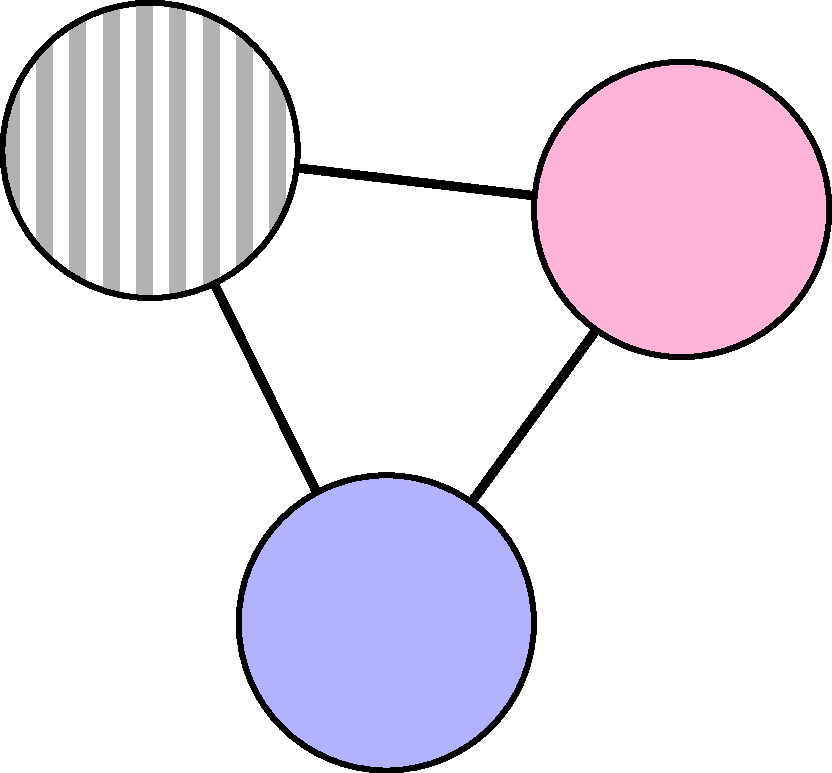
\includegraphics[width=1\textwidth]{puzzle_1.pdf}
      \vspace{17mm}
      \caption{A simple section of the ``AS-graph''.}
    \end{subfigure}
    \hspace{0.05\textwidth}
    \begin{subfigure}[b]{0.54\textwidth}
      \centering
      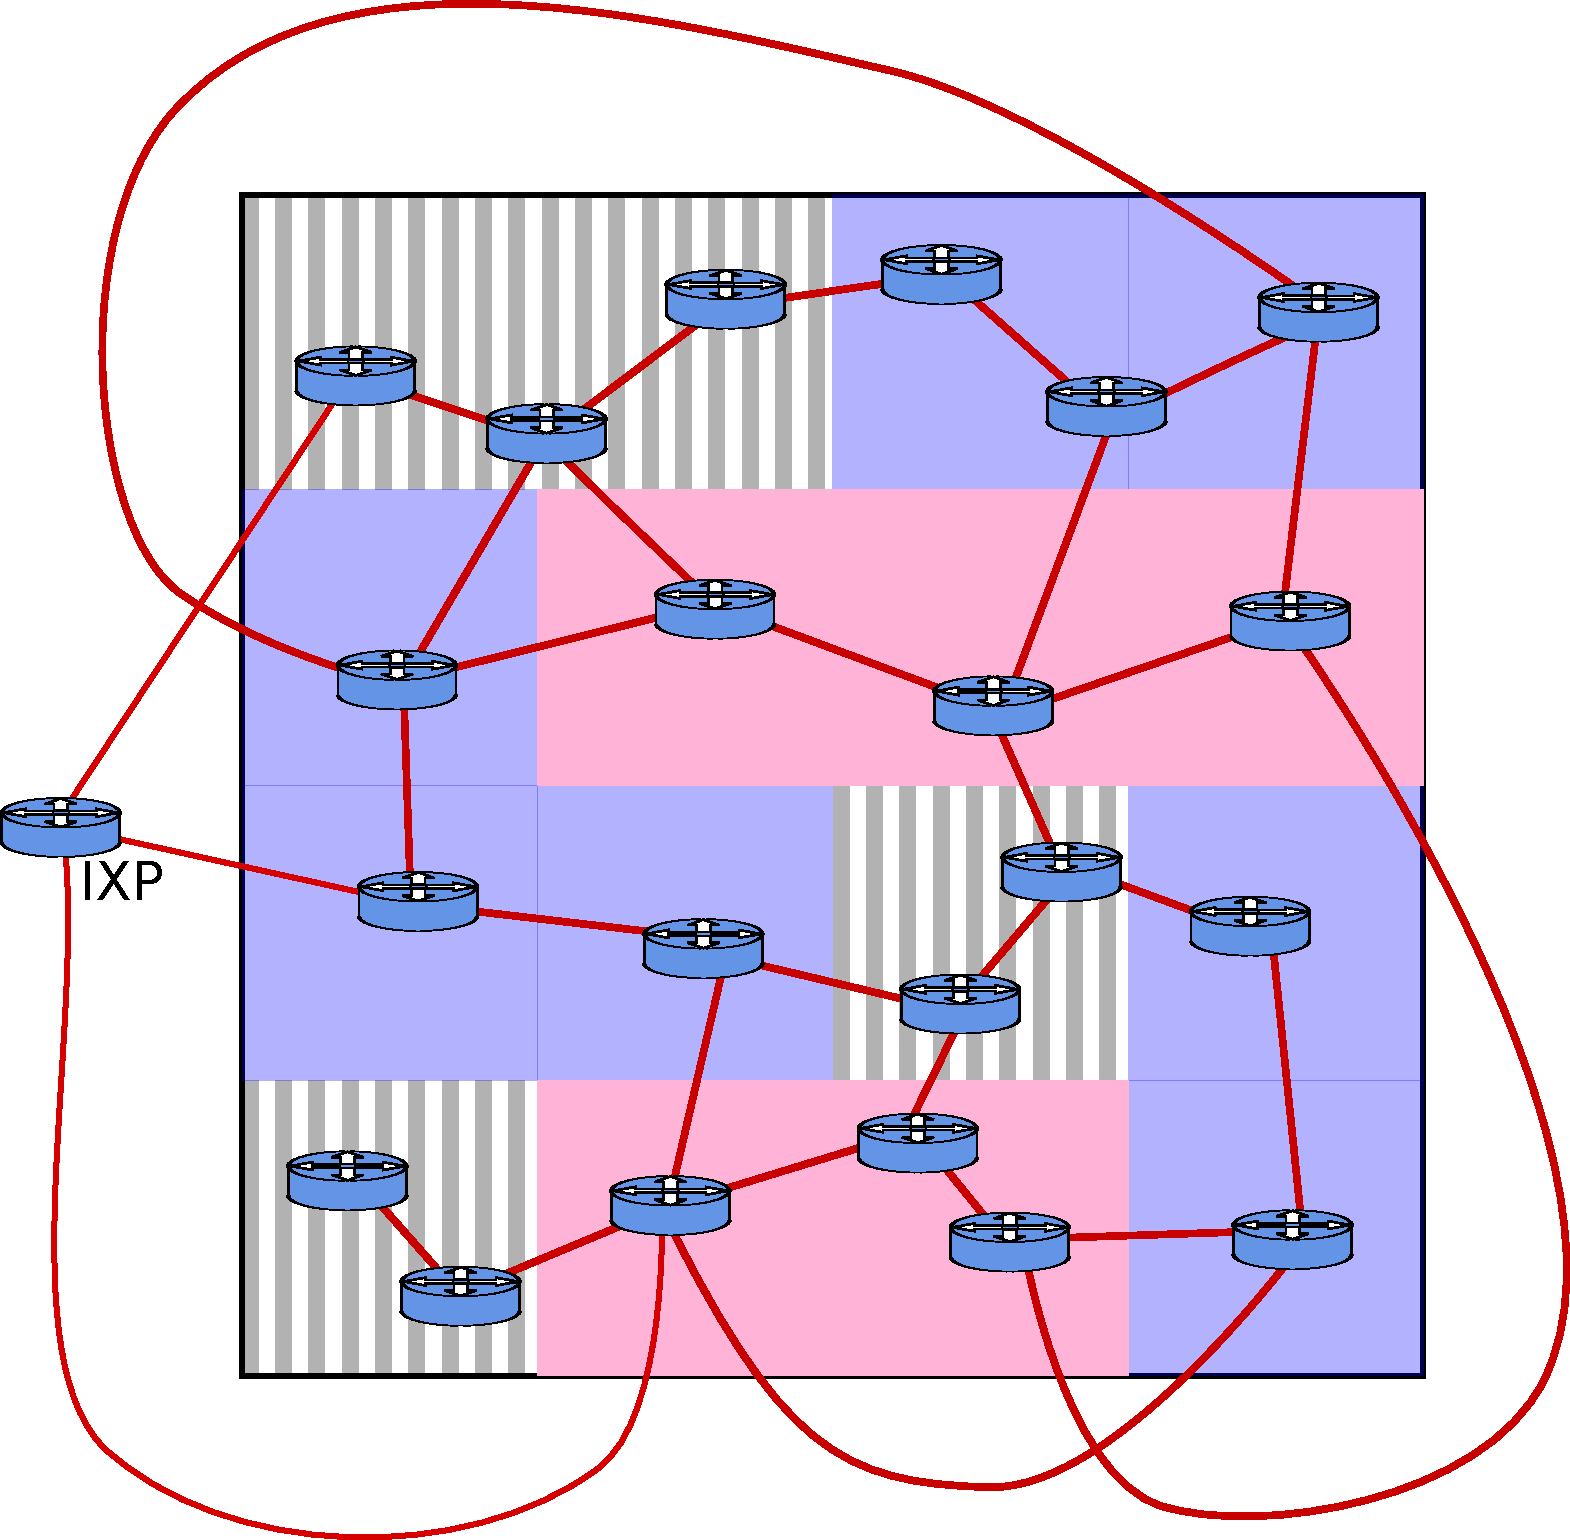
\includegraphics[width=1\textwidth]{puzzle_2.pdf}
      \caption{A possible picture of the router-level connectivity.}
    \end{subfigure}
    \caption{An illustration of the obfuscation of the AS-graph
      (in the vein of \cite{griffin02:_under_border_gatew_protoc_bgp}). The
      graph may appear simple, but hides heterogeneous, non-atomic,
      dis-contiguous entities and interconnects. At the minimum, this
      should illustrate the dangers of talking about the ``Internet''
      graph. \label{fig:puzzle}}
  \end{center}
\end{figure}         

Moreover, the AS-graph treats ASes as nodes, with connecting edges,
but the real situation is much more complex. ASes are complex networks
in their own right, and are connected sometimes by multiple edges
(M{\'e}rindol~\etal~\cite{merindol09:_quant_ases} found that
over half of the ASes they studied were connected by multiple links),
and sometimes through Internet eXchange Points (IXPs) that connect
multiple ASes. In fact, the traditional approach of modeling the
AS-level Internet as a simple connected di-graph is an abstraction
incapable of capturing important facets of the rich semantics of
real-world inter-AS relationships, including different
interconnections for different policies and/or different
interconnection
points~\cite{muehlbauer06:_build_as,muehlbauer07:_in_search}. The
implications of such abstractions need to be recognized before
attributing network-specific meaning to findings derived from the
resulting models.


% In addition to these seemingly trivial, but actually subtle and
% important points of definition, we have those of the level of
% abstraction desired:
% \begin{enumerate}

% \item The commonly-used practice of abstracting ASes to generic atomic
%   nodes without any internal structure is an over-simplification that
%   severely limits our ability to capture critical features associated
%   with real-world ASes such as route diversity, policy diversity, or
%   multi-connectivity.

% \item The traditional approach of modeling the AS-level Internet as a
%   simple connected di-graph is an abstraction incapable of capturing
%   important facets of the rich semantics of real-world inter-AS
%   relationships, including different interconnections for different
%   policies and/or different interconnection points. The implications
%   of such abstractions need to be recognized before attributing
%   network-specific meaning to findings derived from the resulting
%   models.

% \item AS topology as an uninspiring and often meaningless abstract
%   graph towards an approach that views the AS Internet as an economic
%   construct that is constrained by socio-technological factors and is
%   driven by economic incentives and business decisions made by the
%   major players in this area (\eg service and content providers,
%   large corporations, governments).  Although this notion has been
%   advanced by the networking operator community for some
%   time~\cite{norton1,norton_paid_peering,huston99:_peering_i,huston99:_peering_ii},
%   the networking research community has been slow to react and to
%   distance itself from the popular graph view of the inter-domain
%   topology (examples of exceptions
%   include~\cite{chang95,dhamdhere:conext10,labovitz10:_inter_inter_domain_traff}).

% \end{enumerate}


\subsection{Know your measurements}
\label{sec:as_measurement} 

In studying the AS-level Internet, there are some critical differences compared 
to looking at the router-level Internet:

\begin{itemize}

\item No-one ``owns'' the AS structure. There isn't anyone with the type of 
privileged view that a network operator has of its own network. There are 
tens of thousands of ASes, and so we can't reasonably expect to consult all 
of them to collate a picture either.

\item ASes are not ``nodes''. They are complex in their own right, so viewing 
the AS-level Internet as an AS-graph is a big abstraction of reality.

\item Routing between ASes is very different from routing within ASes and 
highlights the difference between graph representations that 
reflect ``reachability" vs. ``connectivity" information.

\end{itemize}

These differences create interesting problems and opportunities for
measurements, some with parallels to the router-level measurement
problems and others without any such parallels.

\subsubsection{Data-plane vs. control-plane measurements}

As discussed in \autoref{sec:router_measurements}, despite all its
deficiencies, traceroute has been the method-of-choice for obtaining
router-level measurements. As a prime example of an active measurement
tool that is confined to the data plane (\ie probe packets take the
same paths as generic data packets), traceroute has also been used to
obtain information about the AS topology but has additional problems
in this domain.

Apart from the already problematic issues (\eg load-balancing,
aliasing, missing data), IP addresses along traceroute paths must now
be mapped to ASes.  This mapping is even harder than the mapping to
routers, not just because the data for doing so is inaccurate or
incomplete (\eg IP to organization allocations may not work because
an organization does not directly correspond to an AS), but also
because the border of an AS is not well-defined in terms of IP
addresses. It is common for a link between two ASes to come from a
subnet allocated by one of the ASes, resulting in an interface in the
other network with an address that is not its
own~\cite{mao03:_as-tr,marchetta13:_detec_third_addres_tracer_traces}.
The problem is further complicated by variations such as anycast or
Multiple Origin ASes \cite{Zhao01:_MOAS}, which provide yet another
set of counter-examples to a straight-forward mapping between AS and
address space. Some work has concentrated on trying to improve the
mapping \cite{pansiot10:_extrac}, and these represent technical
advances, but it is important to understand that the fundamental
difficultly lies in the fact that the boundaries of the ``business''
are not equivalent to the AS boundaries.
 
The other major alternative to obtaining information about the AS topology is 
to collect control plane data in the form of directly measured routing information.  
The primary example of such control plane data are BGP-derived measurements. 
BGP is a path-vector routing protocol, and as such each node transmits
to its neighbors information about the {\em best} path that it knows to 
a destination. Each node then takes the information it has received about 
best paths, and computes its own best path, which it transmits to its neighbors.  
A route monitor receives this information as would any router, and from the 
transmitted path information, can infer links between ASes.  The two best known 
projects that rely on BGP route monitors, Oregon RouteViews~\cite{ORVdata}, 
and RIPE (R\'{e}seaux IP Europ\'{e}ens)'s Routing Information Service~\cite{RIPEdata} 
both use this approach, and each connects to a few dozen different ASes.

However, by its very design, BGP is an information-hiding rather than an 
information-revealing routing protocol. In addition, by its very design, 
BGP is all about reachability and {\bf not} connectivity.  Using it for 
mapping the Internet inter-domain topology is a ``hack'', and so it should 
come as no surprise that it has its own set of problems, including the following:

\begin{itemize}

\item The AS-path information in the announcements is primarily
included for loop detection and does not have to correspond to
reality. It is easy (and not uncommon) to insert additional ASes into 
a path for various purposes, \eg traffic engineering or
measurement~\cite{colitti06:_poison,bush09:_inter_optom}, and
moreover, the AS-path does not have to represent the data path.

\item Path-vector protocols do not transmit information on every path 
in the network. For instance, backup paths may never appear in any 
routing announcements (unless there is a failure), and so may not be 
seen by a route monitor.

\item Path-vector protocols only transmit ``best'' paths, and so there 
is a large loss of visibility from any one viewpoint. It is sometimes 
argued that a large number of viewpoints would
alleviate this, but the viewpoint locations are highly biased
towards larger networks, and this known ``vantage point problem" 
severely biases the possible views of the network~\cite{roughan08:_bigfoot}. 

\end{itemize}

The BGP measurement data being provided by RIPE and RouteViews was originally 
intended to help debug networks, not for mapping. While this data collections 
have been invaluable for that intended original purpose, it is unsurprising 
that it is inadequate when used for a rather different purpose such as mapping 
the AS Internet. However, when this aspect is carefully taken into account, 
good work can be done but requires a critical evaluation of the data.  Problems 
arise primarily when this data is used uncritically.  Other useful sources of 
AS-level measurements such as looking glass servers and route registries suffer 
from similar problems~\cite{Mahadevan06,he07}, and do so for similar reasons: 
they weren't intended to draw a map of the AS Internet.

\subsubsection{Attribute discovery}

The AS topology may be interesting to scientists in itself, but to be useful 
to network engineers, the routing policies that accompany it should also be known.  
It has been common to approximate the range of policies between ASes by a simple 
set of three relationships: (a) customer-provider, (b) peer-peer, and (c) siblings.  
This reduction was at least in part motivated by Huston~\cite{huston99:_peering_i,huston99:_peering_ii} and has been used in various places
\cite{subramanian02:_charac_inter,wang03:_infer,xia04:_as}.  While many 
relationships fall into these three categories, there are frequent exceptions~\cite{hyun03:_tracer_and_bgp,muehlbauer06:_build_as,Qiu07}, for instance, in the form 
of partial transit in a particular region~\cite{maz:partial-transit,norton1}.

Forgetting for the moment the simplification in assuming all policies fit this 
model and the simplifications the AS-graph itself makes, the relationships can 
be represented in the graph by providing simple labels for each edge. Typically, 
the next step after inferring network topology is to infer policies between ASes. 
The most common approach to this problem is to assume the universality of the peer-peer, 
customer-provider, sibling-sibling model, and to infer the policies by finding an 
allocation of policies consistent with the observed
routing~\cite{gao_inferring,xia04:_as,wang03:_infer,battista_inferring:2003,dimitropoulos07:_as_relat}. 

Once relationships are established, a seemingly reasonable next step
is to estimate the hierarchical structure as in
\cite{subramanian02:_charac_inter}. However, the effect of large
numbers of (biased) missing links has not really been considered in
these algorithms.  In fact, the tier structure of the Internet seems
to be largely an illusion. Recent work has shown that there is little
value in the model at
present~\cite{gill08:_flatt_inter_topol,labovitz10:_inter_inter_domain_traff};
but, in contrast to the claims of these papers, there is no strong
evidence that the situation has actually changed or that the tier
model was ever a good model (except maybe in the early stage of the
``public" Internet in the latter 20th century) particularly in light
of the problems in the data.

Alternatively, we can infer a generic set of policies consistent with
routing observations using a more detailed set of routing
measurements~\cite{path_inference_sigmetrics:2005,muehlbauer06:_build_as}
and estimate performance by comparing predicted routes to real routes
(held back from the inference process).


\subsubsection{The ``missing link" problem: Extent and impact}

Perhaps the most obvious problem that results from relying on BGP measurement 
data to map the AS-level Internet is that there are many missing links in the 
resulting AS-graph.  To illustrate the extent of this problem, years of 
concentrated research efforts that relied on a combination of improved inference methods and additional data sources~\cite{chang04:_towards,zhang05:_collec_inter_as_topol,muehlbauer06:_build_as,dimitropoulos07:_as_relat,he07,he09:_lord_of_links,roughan08:_bigfoot,augustin09:_ixps,chen09:_sidewalk,oliveira10:_incompl_of_obser_inter,dhamdhere11:_twelv_years_evolut_inter_ecosy,sanchez13:_dasu}
have produced a picture of the Internet's AS topology that --- as of 
2011 --- consisted of some 35,000-40,000 ASes (nodes) and about 115,000-135,000 
edges (AS links), with about 80,000-90,000 of them being of the customer-provider type and 
35,000-45,000 of the peer-peer type.

More recently, this supposedly up-to-date and most complete view of
the AS-level Internet changed drastically thanks
to~\cite{ager12:_anatom_europ_ixp} that relied on ground truth data
from one of the largest IXPs in Europe (and worldwide) that had at the
time of this study almost 400 member ASes. The main finding of this
recent study is that in this single location, the number of actively
used AS links of the peer-peer type was more the 50,000 --- larger
than the number of all AS links of the peer-peer type in the entire
Internet known as of 2011. Moreover, being extremely conservative when
extrapolating from this IXP to the Internet as a whole,
\cite{ager12:_anatom_europ_ixp} shows that there are easily more than
200,000 AS links of the peer-peer type in the entire Internet, more
than twice the number of all AS links of the customer-provider type
Internet-wide.  Importantly, the main reason for this abundance of AS
links of the peer-peer type at IXPs is well understood --- many IXPs,
especially the larger ones, offer as free service to their member ASes
the use of their route server. This service greatly facilitates the
establishment of peer-peer links between the members of an IXP and has
become enormously popular with members that have an ``open" (as
compared to restrictive or selective) peering policy. Especially for
the larger IXPs, such networks typically constitute the vast majority
of IXP member ASes. \autoref{fig:ixp} provides an illustration of the
connectivity through this IXP and shows that a majority of its member
ASes have an open peering policy (some 300+ members) and establish AS
links of the peer-peer type with one another.

\begin{figure}[thbp] 
  \begin{center}
% pdfimages gets actual 'images' (bitmaps) out of the PDF, but not plots
%  pdfjam p163-ager.pdf  '7' --outfile p163-ager-p7.pdf 
%     extracts a particular page so I can use it here
    \includegraphics*[width=0.65\columnwidth,viewport=77mm 225mm 133mm 270mm]{p163-ager-p7.pdf}
%                                                    xleft ybottom xright ytop
%                                                 a4 = 0 0 210 297
    \caption{Scatter-plot of number of peers per member, based on a
      classification of the member ASes in the four business
      categories defined above: LISP (Large ISP), SISP (Small ISP),
      HCDN (Hosting/service and Content Distribution Network)), and
      AEN (Academic and Enterprise Networks), and by tier.  
      (Reprinted from \cite{ager12:_anatom_europ_ixp}; \copyright 2012 ACM, Inc. Included here by permission.)
      \label{fig:ixp}}
  \end{center}
\end{figure}         

In short, for many years, researchers have worked with AS-graphs that are typically complete 
in terms of nodes, but easily miss more than half the edges. Importantly, these graphs 
have generally a 2:1 ratio of customer-provider type vs. peer-peer type links when 
a 1:3 ratio is much more likely to reflect Internet reality. Clearly, for gaining 
any economic-based understanding of the AS Internet, getting that ratio approximately 
correct is paramount because it is directly impacting how money flows in the 
Internet --- while in a customer-provider relationship, the former pays the latter 
for bandwidth, peer-peer relationships are typically settlement-free (\ie no 
money is exchanged between the involved parties).  

Besides their immediate economic impact, the above missing edges cause also 
significant problems in inferring the AS graph. For instance, it is a requirement 
that a network be multi-homed to obtain an ASN. This means the AS needs to intent 
to connect to at least two upstream providers. In this sense a ``single-homed stub-AS''
does not exist.  Without any doubt, there are exceptions to this rule. However, the 
second link is often a backup link which is invisible to BGP outside of the immediate 
connection, because of BGP's information hiding\footnote{Note that complex BGP policies 
may play a role in this as well~\cite{cost_community,tim:wedgies}.}. Thus, it may 
appear as if a large number of ASes are single-homed stubs.

In \cite{oliveira10:_incompl_of_obser_inter}, the authors separate the missing 
links into {\em hidden} and {\em invisible}.  Whereas the latter are links that 
are missing from the data for structural reasons (\ie it is not just a question 
of quantity (\ie numbers of monitors) but quality (\ie location of monitor)), 
the {\em hidden} links may be found with enough measurements (over time, or 
multiple viewpoints). In \cite{roughan08:_bigfoot} the authors extend that by 
dividing links into a number of classes based on their observability.

The ``missing link" problem in the AS context is much more serious than if those 
links were ``missing at random''.  In particular, the bias in the type of links 
that are missing~\cite{roughan08:_bigfoot} is critical when calculating some 
metrics on the graph, such as distances, precisely because such links are often 
{\em designed} to cut down on the number of ASes traffic must traverse. The 
missing data is also crucial for understanding reliability: for instance, papers 
such as \cite{barabasi00} that argue that high-degree nodes create
vulnerabilities in the Internet ignore the backup links that are invisible in 
these dataset, but obviously crucial when studying the resilience of the network.

\subsection{The Internet's AS-level topologies}

Despite the limitations of measurements, there is a considerable
amount known about the AS-level topology of the Internet, and we talk
here about the issues in defining and modelling that topology.  We
have seen that the definition of an AS is fraught with
problems. Assuming for the time being that the concept of an AS is
well defined so that it makes sense to equate each AS with a node in a
graph, then what is the set of links?  Unfortunately, the question of
which ASes are ``adjacent'' also has no simple answer, and defining
the meaning of a ``link'' between two ASes requires further
consideration.

Does a link mean the ASes have a business relationship, physical
connectivity, connecting BGP session, or that they share traffic? All
the above are reasonable definitions, and none are equivalent. A
common definition is that two ASes are said to be connected (at a
particular time), if they can exchange routing data (and presumably IP
traffic) without the help of an intermediary AS that provides {\em
  transit}. However, this says little about the true business
relationships that are sometimes discussed as a matter of course when
the AS-graph is considered. Moreover, this abstraction looses
considerable information. In reality there are multiple topologies we
want to model, each with its own meaning, structure, potential
applications, and inference problems.

\begin{itemize}

\item {\em Business relationship graph:} in its simplest form this
  graph simply indicates (by an edge) that a business relationship
  exists between the corporations that own two ASNs. Edges could be
  usefully labelled by the type of business relationship, and we list
  a small subset of the possible relationships in
  \autoref{tab:as_graph_set}.

\item {\em Physical link-level graph:} this graph indicates whether
  two ASNs have a physical (layer 1) connection, and how many such
  connections they have. The multiple nature of such connections leads
  this to being a multigraph, as it is very common for two ASes to be
  connected by multiple links and in different geographic locations
  \cite{norton_paid_peering,liljenstam03:_devel_of_inter_backb_topol,spring03:_inflation}. 
  The idea is clearly illustrated by Figure~1 in
  \cite{liljenstam03:_devel_of_inter_backb_topol}, which shows a
  ``pancake'' diagram of the North American Internet backbone. Perhaps
  the reason this critical aspect of the topology is typically ignored
  is that it is very hard to measure---BGP monitor data is in general blind
  to this facet of the topology.
% Traceroutes can show more detail, but suffer from their own problems.
  In addition, this graph should really be a hypergraph. A single
  ``edge'' can connect multiple ASes, for example through an IXP
  \cite{hyun03:_tracer_and_bgp,xu04:_ixps,augustin09:_ixps}. One might
  argue that they are joined by a switch/router, each using
  point-to-point links, but in at least some cases, that switch has no
  place in a AS graph (\ie it has no ASN).  The graph's edges could
  be usefully annotated with link capacity and potentially other
  features such as geographic location.

\item {\em Connectivity graph:} this graph indicates that layer-2
  connectivity exists between two ASNs. In many cases the layer-2
  connectivity between ASNs would be congruent with the layer-1
  connectivity, but with recent advances in network virtualization this
  may not hold for long~\cite{vroom}. 

\item {\em BGP routing graph:} the edges in this graph indicate pairs
  of ASes that have an active BGP session exchanging routing
  information (\ie a BGP session that is in the `established' state~\cite{RFC4271}).

\item {\em Policy graph:}  the edges in this graph are the same as
  those in the BGP routing graph, but include directed policy
  annotations~\cite{tim10:ssp}. We define this separately from the BGP routing graph
  because it may require a multigraph to allow for policy differences
  between different regions. 

\item {\em Traffic graph:} it is the same as the BGP routing graph,
  but the edges are annotated with the amount of traffic exchanged
  between the corresponding ASes.

\end{itemize} 

This is hardly a complete set of possibilities, but already we can see
the potential complexity here. Nevertheless, it appears unusual for studies to
even define precisely what graph they examine (exceptions being papers
such as \cite{govindan97:_topology,oliveira10:_incompl_of_obser_inter}
where the BGP routing graph is explicitly considered).  In
\autoref{tab:as_graph_set}, we list some of the possible graphs, and
their basic properties.  There is no clean 1:1 mapping between
``network'' and ``organization'' and ``AS''
\cite{hyun03:_tracer_and_bgp,cai10:_AS_to_organ_map}, and so it is
highly non-trivial to map between these graphs, and they are certainly
not equivalent.


\begin{table*}[t]
\begin{center}
  \begin{tabular}{|l|l|l|}
    \hline 
    Graph & Edge Annotation & Graph Type \\
    \hline 
    business relationship & subsidiary, partner, customer,... & directed graph \\
    physical link-level & link capacity & multi- hyper-graph \\
    connectivity graph & - & multigraph \\
    BGP routing graph & - & undirected graph \\
    policy graph & BGP policies & directed multigraph \\
    traffic graph & traffic volumes & directed graph \\
     \hline 
  \end{tabular}
  \caption{Example elements of the set of AS graphs.}
  \label{tab:as_graph_set}
\end{center}
\end{table*}


% It should also be clear by now that ASes are not atomic, they are
% geographically distributed entities \cite{rasti10:_eyebal_ases},
% comprised of multiple components distributed over some area of
% space. In principle (according to the RFCs) the AS should have one
% routing policy. Not only is it not exactly clear what this means, but
% it is clearly not
% true~\cite{hyun03:_tracer_and_bgp,muehlbauer06:_build_as,bush09:_inter_optom}.
% The components of an AS may not even be contiguous. An AS may rely on
% a provider AS for transit of its traffic between multiple otherwise
% disconnected components.


\subsection{A look ahead}

Given our list of problems described here, one might be tempted to
think that the AS-graph and routing data in general are useless until
these datasets are drastically improved. However, apart from their
operational utility, RouteViews and RIPE RIS have provided the
essential ingredients for many important studies that match those
services' goals~\cite{RISgoals}. A number of these studies have
improved the Internet significantly, and in the majority of such
successful papers there is no need to exploit the ``graph'' view of
the network. Examples include: (a) The discovery of slow convergence
and persistence oscillation in routing
protocols~\cite{varadhan96:_oscillation,labovitzSig97,labovitzInfo99,labovtizFTCS99,labovitzSig00,govindanNetworks00,griffin02:_analy_med_oscil_probl_bgp}. (b)
Understanding of the impacts (positive and negative) of route flap
dampening~\cite{mao02:_flap,pelsser:rfd}. (c) Determining how much
address space and how many ASNs are being actively
used~\cite{address_space_growth}. (d) Looking for routing ``Bogons''
often related to Internet address hijacking
%\footnote{Hijacking is becoming a potentially destructive problem. See the recent incident with China Telecom \cite{chinahijacking}.}
\cite{ramachandran06:_spam,cymru,hijacking,nick-bogon,chinahijacking}. (e) Debugging
network
problems~\cite{bush07:_testin,feldmann04:_bgp,roughan04:_SNMP_BGPb}.

On the measurement side, there have also been many advancements
towards improving our view of AS topology. For instance:

\begin{enumerate}

\item As BGP routing changes, often
  multiple potential paths are explored and these paths (which are
  unlikely to actually be used as a final choice) can show some of the
  alternative routes available in the
  network~\cite{zhang05:_collec_inter_as_topol}, and thus a more
  complete topology.

\item Missing edges can be found using additional datasets, \eg RIRs
  and looking glasses~\cite{chang04:_towards,zhang05:_collec_inter_as_topol,he07,he09:_lord_of_links},
  or IXP data~\cite{he07,he09:_lord_of_links,augustin09:_ixps,sanchez13:_dasu},
  though care must be exercised with any additional dataset.

\item A routing beacon~\cite{labovitzSig97,mao03:_bgp_beacon,bush09:_inter_optom}
  is just a router that advertises and withdraws
  certain prefixes on a regular schedule. Examination of the observed
  announcements and withdrawals by various route monitors then allows
  estimates of protocol behavior such as convergence time. 

\item Route poisoning prevents announcement from reaching
  certain parts of the Internet. As with beacons, it allows one to
  examine the behavior of BGP in a more controlled manner. This is perhaps 
  the only way to see (some) backup paths, or to understand whether an ISP uses default
  routing~\cite{colitti06:_poison,bush09:_inter_optom}.

\item There are also attempts to not just estimate the topology
  but derive some quality measure for the resultant
  AS-graph~\cite{inter_as_level_topol_const_analy,winter09:_model_inter_routin_topol_with,roughan08:_bigfoot}.
 
\end{enumerate}

There is often an unfortunate side-effect to some of these types of measurement in
form of a Heisenberg-like uncertainty principle. That is, it is not clear
whether observed changes are due to the micro-phenomenon of path
exploration or macro-phenomena of link changes, new entrants, etc.
The longer we make observations, the more complete they may seem,
but we then do not know whether all of those links existed at the
same time. Such uncertainty principles appear to be present in a
number of Internet measurement contexts~\cite{roughan05:_fundamental} 
where we trade off ``accuracy'' of the measurements against ``time localization''.
In any case, this approach does not overcome the structural bias mentioned earlier. 

At the same time, the above-mentioned and other advances on the measurement side
suggest that the missing link problem may be improved, providing
``more complete'' AS graphs. However, there is a profound need
(illustrated by the above) for better data accuracy measurements, and
better response to data quality issues from subsequent users of the
data. Obvious ways to improve are to conduct sensitivity analysis (of
results) to missing or incorrect input data. 

In addition, it is to be hoped that more controlled experiments are
conducted (\ie experiments that have a ``control'' sample against
which the experimental data can be compared) in order to precisely
derive which factors of interest affect which variables.  Controls
allow one to discriminate alternative explanations for results, and
prevent the affects of one confounding factor drowning out the affects
of others (see \cite{mao03:_bgp_beacon,bush09:_inter_optom}). This is
basic tenet of the scientific method, but seems to have been ignored
in this area of research. Most studies have been ``observational'',
and while there is a valid role for such experiments, for instance in
epidemiology, they are intrinsically harder to interpret.

Lastly, another aspect of this richer set of AS topologies is that it should be
obvious by now that economic or commercial objectives by and large determine
and shape the structure and evolution of their real-world counterparts, and that 
these constructs are once again naturally expressed through optimization rather 
than random graph models, though in this case the optimization problems may come
from game theory or economics rather than mathematical programming. 

\subsection{Notes}

The primary sources for the material presented in this section are

\begin{itemize}

\item[\cite{roughan11}] M. Roughan, W. Willinger, O. Maennel,
D. Perouli, and R. Bush. 10 Lessons from 10 Years of Measuring and Modeling the Internet's Autonomous Systems, in: {\em IEEE Journal on Selected Areas in Communications} 29(9):1810-1821, 2011.

\item[\cite{ager12:_anatom_europ_ixp}] B. Ager, N. Chatzis,
A. Feldmann, N. Sarrar, S. Uhlig, and W. Willinger. Anatomy of a
large European IXP, in: {\em Proc. ACM SIGCOMM'12, ACM Computer
Communication Review} 42(4), 2012.

\end{itemize}
and they contain lengthier discussions of many of the issues touched upon here. 

For additional and more in-depth reading materials (in
addition to the references indicated throughout) we point to

\begin{itemize}

\item[\cite{chang-thesis06}] H. Chang. Modeling the Internet's
Inter-Domain Topology and Traffic Demand Based on Internet Business Characterization, PhD Thesis, University of Michigan, 2006.

\item[\cite{Donnet07}] B.Donnet and  T. Friedman, Internet Topology Discovery: A Survey, IEEE Communications Surveys \& Tutorials, 9(4), pp.56-69, 2007.

\item[\cite{dhamdhere-thesis08}] A. Dhamdhere. Understanding the
Evolution of the AS-level Internet Ecosystem, PhD Thesis, Georgia Institute of Technology, 2008.

\item[\cite{haddadi08:_networ_topol}] H. Haddadi, M. Rio,
G. Iannaccone, A. Moore and R. Mortier, Network topologies:
inference, modeling and generation, IEEE Communications Surveys,
10(2), 2008.

\item[\cite{dhamdhere11:_twelv_years_evolut_inter_ecosy}] A. Dhamdhere
  and C. Dovrolis. Twelve Years in the Evolution of the Internet
  Ecosystem, in: {\em IEEE/ACM Transactions on Networking} 19(5),
  2011.

\end{itemize}

\clearpage
\section{PoP-level topology}


When designing or reconfiguring the physical infrastructure of an ISP, network 
operators are often guided by a design principle that emphasizes 
{\em hierarchy}~\cite{Cisco05,Gill,Morris07}.  There are two main reasons 
for implementing hierarchical network designs: {\em scalability} and {\em simplicity}.  
Compared to non-hierarchical designs, hierarchical networks can often be built at scale, 
mainly because hierarchy makes a network easier to visualize --- a key feature towards 
making it easier to manage. The situation is analogous to modularity in programming 
languages --- ideally it allows consideration of network components in isolation.

A common form of hierarchy in IP networks is based on the concept of the PoP (or 
Point of Presence). A PoP is a loosely defined term. Some providers may use the 
term to mean a physical building (housing a group of routers, switches and other 
devices), whereas others mean a metropolitan area where service is provided. 
However it is defined, though, it is a useful construct because it describes 
the logical structure of the network as the designer intended, rather than its 
particular implementation in terms of individual routers. Moreover, irrespective 
of the meaning, PoPs have an explicit geography (\eg street address or 
city/metropolitan area).  This then leads to our third major category 
of ``Internet topology'' --- the PoP-level topology.

PoP-level topologies are ideal for understanding tradeoffs between connectivity 
and redundancy, and also provide the most essential information to competitors 
or customers (about where a network is based, or who has the best access network 
in a region).  Additional reasons why the PoP-level view of networks is interesting 
include

\begin{itemize}

\item Network maps are often drawn at this level because it is an easy level 
for humans to comprehend.

\item Network optimization is often conducted at this level because the problem 
size is generally reasonable (\eg dozens of PoPs as compared to potentially 
hundreds of routers) and because inter-PoP links are much more expensive than 
intra-PoP links.

\item The internal design of PoPs is almost completely determined by simple 
templates \cite{Cisco05,Gill,Morris07}.

\item Networks change less frequently at the PoP level than at the router 
level~\cite{Shavitt10}; and

\item The PoP level is the more interesting level for many activities because 
it is less dependent on the details of protocol implementations, router vendor 
and model, and other technological details.

\end{itemize}

\begin{figure}[!thbp] 
  \begin{center}
    \begin{subfigure}[b]{0.58\textwidth}
      \centering
      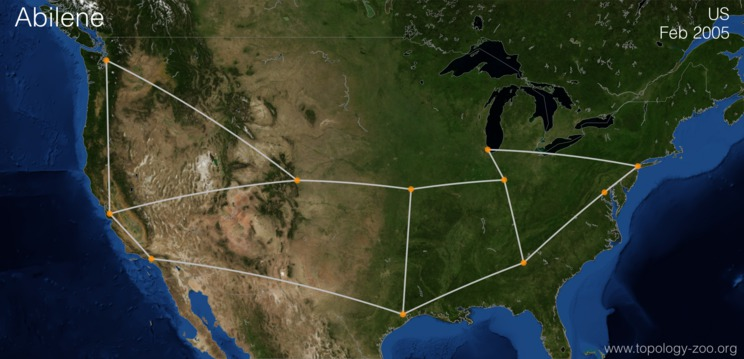
\includegraphics[width=1\textwidth]{Abilene.jpg}
    \end{subfigure}
    \hspace{0.02\textwidth}
    \begin{subfigure}[b]{0.38\textwidth}
      \centering
    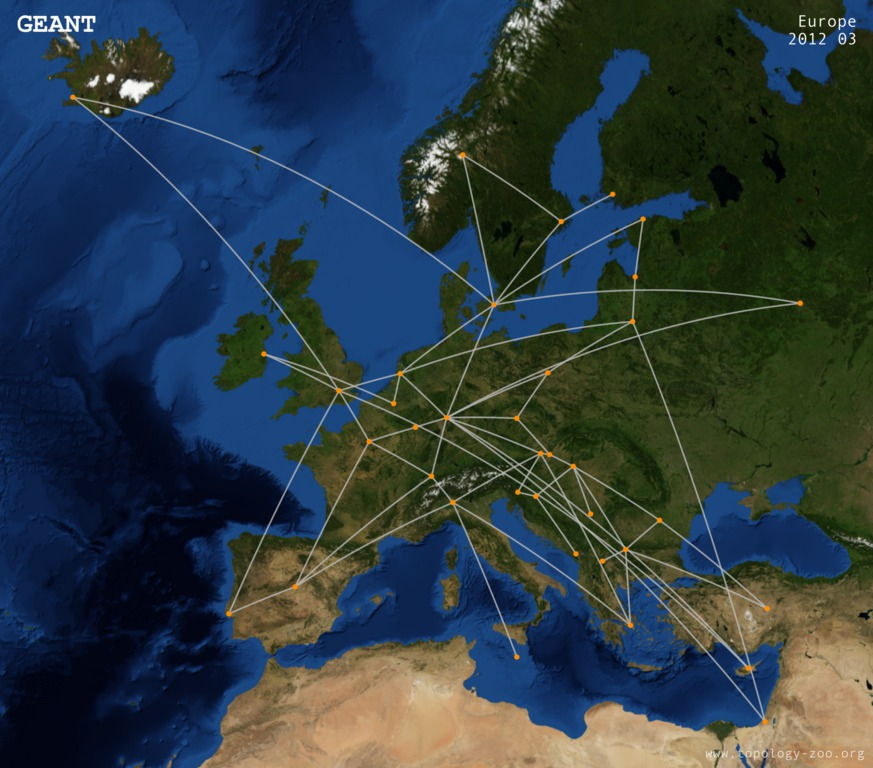
\includegraphics[width=1\columnwidth]{Geant2012.jpg}
    \end{subfigure}
    \caption{PoP-level network topologies taken from \url{www.topology-zoo.org}.
      \label{fig:pop}}
  \end{center}
\end{figure}         

The last point is subtle but important for modelling. For instance, when using a 
network as part of a simulation, one would like to have a network that is 
{\em invariant} to the method being tested. If a network designer might change 
his/her network in response to a new protocol, say a routing or traffic engineering 
algorithm, then the test will be ambiguous if it uses existing networks as models. 
PoP-level networks are less sensitive to these details than router-level networks, 
because routers impose physical and technological constraints that are almost 
completely dependent on the details of the router vendor, model and even the 
version of software running on the router.

Two examples of PoP-level topologies are depicted in \autoref{fig:pop}, 
showing the structure of two of the largest research networks (Abilene, 
and G\'{E}ANT) in the world. 

\subsection{A look back}

The study of PoP-level topologies has a briefer history than the major 
alternatives. Although the concept has existed for almost as long as networks, 
the work on modelling and measurement has typically focussed on routers (or 
their equivalent) though it is noteworthy that in simple networks (with one 
router per PoP) the two are the same. 

The first steps were taken when real data-networks were observed and
it was noted that they had structure in the form of hierarchy that was
not well represented in simple random graphs.  This observation led to
the development of \emph{structural topology
  generators}\cite{Zegura97}, based on the idea that a topology
generator should reflect the obvious hierarchical structures visible
in real networks (\eg the Georgia Tech Internetwork Topology Models
(GT-ITM)~\cite{GTITM} generator). However, this model was not
specifically aimed at modelling the PoP-level.  PoPs have been used in
more advanced structural topology generators such as
IGen~\cite{quoitin09:_igen}. IGen explicitly treats network design as
an optimization, rather than following simple stochastic rules, in
order to mimic the manner in which real networks are designed.  IGen
uses this not only for topology but also to create some of the other
important details of the network, such as the link metrics or iBGP
configurations.

The Rocketfuel project~\cite{rocketfuel_1} sought to measure (using traceroute 
with all the problems described earlier) individual ISPs, and as part of this, 
presented data and maps at the PoP level. The idea was extended by the iPlane 
project \cite{iPlane}, and by DIMES
\cite{Shavitt:2012:GIP:2238856.2238872}. However, the flaws in
traceroute make this data and the ensuing maps suspect from the start. 
However, \cite{rocketfuel_1} raised the bar with respect to validating the 
obtained PoP-level maps by trying to solicit feedback from the operators in 
charge of the mapped ISPs. 

More recently, the concept of a PoP has been explicitly used to help
guide measurement approaches, in the hope to overcome some of the
limitations of traceroute~\cite{Feldman08,Yoshida09,Shavitt10}.
However, in the absence of strong validation and given traceroute's
many problems, it is likely that most of the known issues still exist
in these approaches.

Alternatively, Knight~\etal~\cite{Zoo} have collected a set of over 
200 maps published by ISPs themselves, and transcribed these into an open 
set of data available from \url{www.topology-zoo.org}. Much of this data is 
at the PoP-level, indicating the importance of this level of network 
representation to ISPs. For a similar but complementary effort, see~\cite{atlas}.
 
\subsection{Know your measurements}

The problems in measuring PoPs are essentially the same as in any
traceroute-based survey, though it is thought (or perhaps just hoped)
that mapping IP addresses to PoPs is more straight-forward than
mapping IPs to either routers or to ASes. To the best of our
knowledge, no rigorous testing of this hypothesis has been conducted
to date, but there are some indications (\eg see \cite{Zoo}) that the
PoP-level maps provided by traceroute are no better than their router-
or AS-level counter-parts.

The topology-zoo data~\cite{Zoo}, on the other hand, is provided by
ISPs themselves and should in principle be much more accurate.
However, this dataset must also be treated carefully (as should all
data) because of potential transcription errors, or mistakes or
approximations in the maps provided by the ISPs. While such errors are
much less frequent than those encountered in measured networks, an
added concern with respect to ISP-provided maps is stale data because
there is little incentive to provide up-to-date maps.

As mentioned earlier, another important component of many PoP-level
topologies is the geographic element. Such topologies are much easier
to visualize geographically \cite{knight12:_i}, and so a frequent
interest is geolocation of the PoPs. While this is not a chapter on
geolocation, it suffices to say that many research papers have been
written on the problems of accurately mapping IP addresses to their
geolocation (\eg see \cite{Poese:2011:IGD:1971162.1971171}). Moreover,
while the routers and switches of a PoP are typically located in a
single location, city, or metropolitan area, the ``eyeballs'' (\ie end
users) connected to the PoP will be spread over some
area~\cite{rasti10:_eyebal_ases}.  However, if the researcher is
willing to diligently mine various data sources, there is hope of at
least being able to geolocate PoPs as they house potentially hundreds
or thousands of IP addresses and reside in locations with known
physical addresses (\eg carrier hotels)~\cite{atlas}.


\subsection{The nature of the PoP-level graph}

There is a common meme in network modelling that the design of a US ISP backbone 
network involves simply selecting the NFL cities, and then joining them up with 
a few lines on a map. While the real process of network design is rarely so trite, 
the picture above isn't entirely unfair. 

Most notably, PoPs are usually selected based on commercial criteria (\eg the 
desirability and size of the potential customer base in an area). So network 
engineers get little choice over the locations that they are connecting. They 
could be the NFL cities in the US, or the larger cities of another country, or 
the capitals of countries on a continent, and so on. 
Once the PoP locations have been selected, they need to be connected in some 
redundant fashion to ensure some degree of robustness to node or link failures. 
Historically, connecting these PoPs may have been done in a mostly {\em ad hoc} 
manner; see for instance \url{http://personalpages.manchester.ac.uk/staff/m.dodge/cybergeography/atlas/roberts_arpanet_large.gif}. 

However, since the burst of the Internet bubble ({\em circa} 2000), capital 
investment has become harder to obtain, and network operators and engineers 
had to justify such investment more carefully. At this point, network capacity 
started to be more carefully planned, not always using formal mathematical 
optimization, but certainly using traffic measurements to ensure less wasted 
capacity. Much of this planning and optimization is performed at the PoP-level 
simply because the router-level is much more complicated (in size, and complexity of
constraints), and because inter- and intra-PoP link costs vary by a large margin.

We have discussed network design by constrained optimization extensively in 
\autoref{sec:router} (see also references such as \cite{Li04}), and so here 
we shall only consider the main differences for PoP-level design (apart from 
those already listed above).

Perhaps the most important difference is that the physical and engineering 
constraints on a router do not directly apply for a PoP. At least in theory, 
a PoP can use as many routers as needed to provide sufficient number of ports 
for any arbitrary node degree and sufficient throughput per port. Naturally, 
the constraints in this case will arise in the form of costs, and optimization-based 
formulations of the PoP-level network design problem will feature budget constraints 
to reflect this aspect.  As budget constraints can vary greatly among different 
companies, when we look at actual PoP-level ISP backbone networks, we see a wide 
variety of designs ranging from the meshy designs with high-degree nodes only at 
the edge predicted by the HOT model, to hub and spoke like networks~\cite{Zoo}. 
In fact, the sheer variety of network designs we observe in reality suggest that 
while some network operators seem to aim at optimizing performance (given some 
lenient cost constraints), others appear to be willing to sacrifice performance 
in order to keep costs low. Moreover, network operators in different countries 
can encounter very different link costs depending on the local geographic and 
commercial environment. 

A critical but rarely discussed property of the PoP-level topology is that it 
provides the ``glue" between the more physical router-level topology on the one 
hand and the more logical AS-level topology on the other hand. Functioning as 
an ``intermediary" between these two topologies highlights the important aspect 
of the PoP-level topology that its granularity is ``just right" for many networking 
problems of practical interest --- not too coarse as to ignore important context 
(\eg the case with various AS topologies) but also not too fine as to be 
overwhelmed with unnecessary details (\eg the case with various physical 
topologies). We next discuss this property in more detail.

\subsubsection{From PoP-level to router-level connectivity}

Given a PoP-level network, there is an additional interesting
question: ``Can we map this network down to the router level?''  The
GT-ITM model addressed this through random generation of its
subnetworks, but in practice the design process of network engineers
in this case is a text-book application of repeating
patterns~\cite{Cisco05,Gill,Morris07} and hence anything but random.

The main reason for following this design process is that network 
designers often apply ``cookie cutter'' methods to design networks as a whole
or the internals of PoPs, though that term unnecessarily
trivializes the importance of repeated patterns. Repetition makes
network operations vastly simpler: the management of two PoPs requires
the same skills.  Equipment can be bulk purchased, debugging is
easier, and adding new PoPs is simpler. Finally, networks based on
templated design lead to simple design methodologies. For instance,
the inter-PoP level network topology can be optimized relatively
simply, as details such as redundancy will be supplied by the
provision of pairs of redundant routers in each PoP, with redundant
links between them.  Design often refers to the graph topology of
router interconnections, but templated design can extend to other
details, such as physical configuration within racks, connections with
external networks, or additional servers such as Domain Name Service
or Network Management Systems. 

This type of design can be mathematically described using
graph-products, though for more details, we invite the reader to consult
\cite{parsonage11:_gener_graph_produc_networ_desig_analy}.


\subsubsection{From PoP-level to AS-level connectivity: The pancake-view of the Internet}

Until now we have only really discussed the PoP-level topology of a
single network. However, there is considerable interest in how these
networks interconnect. 


The most prominent and commonly-accepted view of the Internet is as a
``network of networks'' or ASes in the AS-graph representation
discussed in \autoref{sec:as}.  A much neglected and rarely-mentioned
representation is the ``pancake view'' where we consider each network
to be a layer and where the different layers (networks) are stacked on
top of one another to form a pancake-like
structure~\cite{liljenstam03:_devel_of_inter_backb_topol}. To show
where the different networks inter-connect, we add links across
layers; intra-network connectivity is shown as links within each
layer.  For a set of ``peer'' networks, one advantage of this pancake
view is that these networks often cover similar geographic areas and
inter-connect in multiple locations, but at a limited set of cities
(determined either by where private interconnects are seen as
commercially viable, or where IXPs are available). Importantly,
depending on the types of networks, many of them host their PoPs in
one and the same commercial colocation facilities whose street
addresses are generally known\footnote{One problem in establishing
  such a view lies in the limitations of current IP geolocation
  services \cite{Poese:2011:IGD:1971162.1971171}.}.  As such, the
pancake view allows one to visualize not only this connectivity inside
and between such providers but also the geography of their PoP-level
topologies.

However, as far as we are aware, there has been no significant work
studying this pancake view together with the different inter-connections, 
other than noting that it exists. The dearth of studies and models perhaps 
stems from the problems in obtaining the measurements necessary for constructing
this view (see the discussions in \autoref{sec:as}), but it is
perhaps one of the most interesting areas for future Internet topology research.
 

\subsection{A look ahead}

We have focused in this section and the earlier sections mostly on traditional ISPs
or network service providers which operate networks that have more or
less pronounced backbones and cover geographic areas ranging from 
individual countries to entire geographic regions to the entire globe.
However, there are many other networks that are not ISPs and consist of PoPs
without their own physical infrastructures to connect them (\eg content
providers, CDNs, Web-hosting companies). The PoPs of these networks are
typically located in commercial colocation facilities or data centers
that are operated by third-party companies for the explicit purpose of 
interconnecting such infrastructureless networks among one another or 
with ISPs or network service providers. 

The importance of the role of such dedicated Internet infrastructure
in the form of colocation facilities is best illustrated with a
concrete example.  As of December 2012, Equinix \url{www.equinix.com},
one of the leading companies in global interconnection and data
centers, owned and operated in 14 countries in 5 continents some 30
colocation facilities. In these 30+ colocation facilities that are
located in the major cities around the world, more than 4,000 networks
connected directly to their customers and partners.

Another largely under-researched topic concerns the fact that in this chapter,
we treated router-, PoP-, and AS-level topologies as static objects, when in
reality, they evolve over time.  In particular, it is rarely the case that
a network operator designs a new network from scratch.  Network design typically
has to include as important aspects awareness and knowledge of the 
existing network that the operator intends to change due to, for example,
drastic changes in the traffic demand that the original network design can
no longer handle efficiently.

In view of these an other added challenges, the PoP-level view promises
to be one of the more useful and interesting direction for future Internet
topology research.  In particular, measurements and models at this level have
considerable scope for the future, and extensions of HOT-like optimization
models may provide much more realistic synthetic networks than are
currently available. At the same time, work on interconnection of networks 
at this level also provides considerable scope, but will require significant
advances in our ability to measure and model the flow of traffic across the
different networks as it is the traffic that ultimately determines much of
the structure and evolution of the different topologies that we discussed 
in this chapter.

\subsection{Notes}

The primary source for the material presented in this section (and a
much lengthier discussion of many of the issues) is

\begin{itemize}
\item[\cite{Zoo}] S.Knight, H.Nguyen, N.Falkner, R.Bowden, M.Roughan,
  The Internet topology zoo. IEEE Journal on Selected Areas in
  Communications (JSAC) 29, 9, 1765-1775, October 2011.

\end{itemize}

\noindent For additional and more in-depth reading materials (in
addition to the references indicated throughout) we point to

\begin{itemize}

\item[\cite{Shavitt:2012:GIP:2238856.2238872}] Y.Shavitt and
  N.Zilberman, Geographical Internet PoP-level maps. In Proceedings of
  the 4th international conference on Traffic Monitoring and Analysis
  (Berlin, Heidelberg), TMA'12, Springer-Verlag, pp. 121-124, 2012.

\item[\cite{parsonage11:_gener_graph_produc_networ_desig_analy}]
  E.Parsonage, H.Nguyen, R.Bowden, K.Knight, N.Falkner, M.Roughan,
  Generalized graph products for network design and analysis. In 19th
  IEEE International Conference on Network Protocols (ICNP)
  (Vancouver, CA), October 2011.

\item[\cite{Shavitt10}] Y.Shavitt and N.Zilberman, A structural
  approach for PoP geo-location. In IEEE Infocom 2010.

\item[\cite{Yoshida09}] K.Yoshida, Y.Kikuchi, M.Yamamoto, Y.Fujii,
  K.Nagami, I.Nakagawa and H.Esaki, Inferring PoP-level ISP topology
  through end-to-end delay measurement. In PAM, pp. 35-44, 2009.

\end{itemize}


% \input{overlay}
%\ed{A one page conclusion.} 
%Something on evolution of transport
%Something on Middleboxes
%Something on MPTCP
%Something on Minion
%One paragraph on the future

The Transport Layer in the Internet evolved for nearly two decades,
but it has been stuck for over a decade now.
A proliferation of middleboxes in the Internet,
devices in the network that look past the IP header,
has shifted the waist of the Internet hourglass 
upward from IP
to include UDP and TCP,
the legacy workhorses of the Internet.
While popular for many
different reasons, 
middleboxes thus deviate from the Internet’s
end-to-end design, creating large deployment
“black-holes”---singularities where legacy transports get through, but
any new transport technology or protocol fails,
severely limiting transport protocol evolution.
The fallout of this ossification
is that new transport protocols,
such as SCTP and DCCP,
that were developed to offer much needed 
richer end-to-end services to applications,
have had trouble getting deployed since they require changes 
to extant middleboxes.

Multipath TCP is perhaps the most significant change to TCP in the past twenty
years. It allows existing TCP applications to achieve better
performance and robustness over today's networks, and it has been
standardized at the IETF. The Linux kernel implementation shows that
these benefits can be obtained in practice.  However, as with any
change to TCP, the deployment bar for Multipath TCP is very high: only
time will tell whether the benefits it brings will outweigh the added
complexity it brings in the end-host stacks.

The design of Multipath TCP has been a lengthy, painful process that took around five
years. Most of the difficulty came from the need to support existing middlebox
behaviors, while offering the exact same service to applications as TCP. Although
the design space seemed wide open in the beginning, in the end we were \emph{just} able
to evolve TCP this way: for many of the design choices there was only one viable option
that could be used. When the next major TCP extension is designed in a network with even more
middleboxes, will we, as a community, be as lucky?

A pragmatic answer to the inability to deploy new transport protocols
is Minion. It allows deploying new transport services 
by being backward compatible with middleboxes by encapsulating new protocols inside TCP.
Minion demonstrates that it is possible to obtain
unordered delivery and multistreaming
from wire-compatible TCP and TLS streams
with surprisingly small changes to TCP stacks
and application-level code.
Minion offers a path toward
the performance benefits of unordered delivery,
which we expect to be useful to applications
that use TCP for a variety of pragmatic reasons.

%Minion is just the latest in an ever-growing encapsulation war that 
%has engulfed end-hosts and network providers for years on end. 
Early in the Internet's history,
all IP packets could travel freely through the Internet, as IP was the narrow waist of
the protocol stack. 
Eventually, 
apps started using UDP and TCP exclusively,
and some, such as Skype, used them adaptively,
probably due to security concerns
in addition to the increasing proliferation of middleboxes that allowed only UDP and TCP through.
As a result, UDP and TCP over IP were then perceived to constitute the new waist of the Internet.
(We'll note that HTTP has also recently
been suggested as the new waist~\cite{popa10http}.) 
%UDP is not that great getting through newer firewalls either, so TCP is the new narrow
%waist, or even HTTP as recently proposed. 

Our observation is that
whatever the new waist is,
middleboxes will embrace it and optimize for it: 
if MPTCP and/or Minion become popular, 
it is likely that middleboxes will be devised that understand these protocols
to optimize for the most successful use-case of these protocols
and to help protect any vulnerable applications using them.
One immediate answer from an application would be to
use the encrypted communication proposed in Minion---%
but actively hiding information from a network operator
can potentially encourage the network operator
to embed middleboxes that intercept encrypted connections,
effectively mounting man-in-the-middle attacks
to control traffic over their network,
as is already being done in several corporate firewalls~\cite{marko10using}.
%a potential serious security breach, and many ISPs
%may either drop traffic or require their customers to ``install'' keys in the 
%browser that effectively allow middleboxes to become a man-in-the-middle of the TLS connection. 
To bypass these middleboxes,
new applications may encapsulate their data {\em even} deeper,
leading to a vicious circle resembling an ``arms race'' for control
over network use.
% them looking even deeper in the packets. As we can see, 
%this is a vicious circle that no-one can ever win.

This ``arms race'' is a symptom of a fundamental tussle between
end-hosts and the network: end-hosts will always want to deploy new
applications and services, while the network will always want to allow and optimize only
existing ones~\cite{tussle}.
To break out of this vicious circle,
we propose that
end-hosts and the network must co-operate,
and that they must build cooperation into their protocols.
Designing and providing protocols and incentives for this cooperation may hold the key to creating a
truly evolvable transport (and Internet) architecture.


%\clearpage
%{
%\setlength{\parskip}{1mm}
%\footnotesize
% \bibliographystyle{ieeetr}

% Define style for bibtex bibliography
\bibliographystyle{../acm}
%\bibliographystyle{acm}  
% http://sites.stat.psu.edu/~surajit/present/bib.htm
% http://www.cs.stir.ac.uk/~kjt/software/latex/showbst.html
% http://en.wikibooks.org/wiki/LaTeX/Bibliography_Management#Bibliography_styles
% \bibliography{cov,books,statistics,routing,internet,graph,bgp,ospf,ip_traffic,measurements,topology_fulllist} 
\bibliography{topology} 
 
%\clearpage
% \printindex
%}

\end{document}


